\documentclass{article}

\usepackage[margin=25mm]{geometry}
\usepackage{amsmath}
\usepackage{array}
\usepackage{amssymb}
\usepackage[hidelinks]{hyperref}
\usepackage[
type={CC},
modifier={by-nc-sa},
version={4.0},
]{doclicense}

\DeclareMathOperator\supp{supp}

\title{List of univariate probability distributions} 
\author{Maximilian L. Grei\ss l}
\date{\today}

\begin{document}
	\maketitle
	\tableofcontents
	\vfill
	\doclicenseThis
	
	\newpage
	
	\section{Discrete distributions}
	This list gives an overview of the most popular univariate probability distributions and their most important properties. \\
	In the following, let $K$ and $X$ denote appropriately distributed discrete and continous random variables, respectively.
	
	\subsection{Discrete uniform($n$) distribution}
	\begin{tabular}{|*2{>{\centering\arraybackslash}p{.48\textwidth}|}}
		\hline
		Mass function 
		\[ f \left ( k \right ) = \frac{1}{n}
		\] 
		& Distribution function
		\[ P\left ( \left \{ K \leq k \right \} \right ) = \frac{|\left \{ i:k_{i}\leq k \right \}|}{n} \]
		\\
		\hline
		Mean
		\[ E\left [ K \right ] = \frac{1}{n}\sum_{i=0}^{n}k_{i} \]
		& Variance
		\[ \text{Var}\left( K\right) = \frac{1}{n}\left ( \sum_{i=0}^{n}k_{i}^{2} -\frac{1}{n}\left ( \sum_{i=0}^{n}k_{i} \right )^{2} \right ) \]
		\\
		\hline
	\end{tabular} \\

	\subsection{Bernoulli($p$) distribution}
	\begin{tabular}{|*2{>{\centering\arraybackslash}p{.48\textwidth}|}}
		\hline
		Mass function 
		\[ f(k)=
		\left\{\begin{matrix}
			p & \text{ for } k = 1\\ 
			1-p & \text{ for } k = 0
		\end{matrix}\right \]
		& Distribution function
		\[ P\left ( \left \{ K \leq k \right \} \right ) = \left\{\begin{matrix}
			0 & \text{ for } k<0 \\ 
			1-p & \text{ for } 0\leq k<1 \\ 
			1 & \text{ for } k\geq 1
		\end{matrix}\right. \]
		\\
		\vspace{-20pt}
		 $\supp f\left( k\right) = \left\lbrace 0,1\right\rbrace $ &
		 \\
	\end{tabular}
	
	\vspace{-12pt}
	\begin{center}
		\begin{tabular}{|*3{>{\centering\arraybackslash}p{.3112\textwidth}|}}
			\hline
			Mean
			\[ E\left [ K \right ] = p \]
			& Variance
			\[ \text{Var}\left( K\right) = p \left( 1-p\right) \] 
			& Fisher Information
			\[\mathcal{I} \left ( \theta \right ) = \frac{1}{\theta\left ( 1 - \theta \right )}\]
			\\
		\end{tabular} \\
	\end{center}
	
	\vspace{-22.5pt}
	\begin{center}
		\begin{tabular}{|*2{>{\centering\arraybackslash}p{.48\textwidth}|}}
			\hline
			Moment-generating function
			\[ M_{X}\left( t\right) = \left(1-p+p\exp\left( t\right)  \right) \]
			& Characteristic function
			\[ \varphi_{X}\left( t\right) = \left(1-p+p\exp\left( it\right)  \right) \]
			\\
			\hline
		\end{tabular} \\
	\end{center}
	
	\newpage
	
	\subsection{Hypergeometric($M$,$N$,$n$) distribution}
	\begin{tabular}{|*2{>{\centering\arraybackslash}p{.48\textwidth}|}}
		\hline
		Mass function 
		\[ f\left ( k \right ) = \frac{\binom{M}{k}\binom{N-M}{n-k}}{\binom{N}{n}} \] 
		& Distribution function
		\[ P\left ( \left \{ K\leq k \right \} \right ) = \sum_{i = \text{max}\left\lbrace  0,n-N \right\rbrace }^{\left \lfloor k \right \rfloor} \frac{\binom{M}{i}\binom{N}{ni}}{\binom{M+N}{n}} \]
		\\
		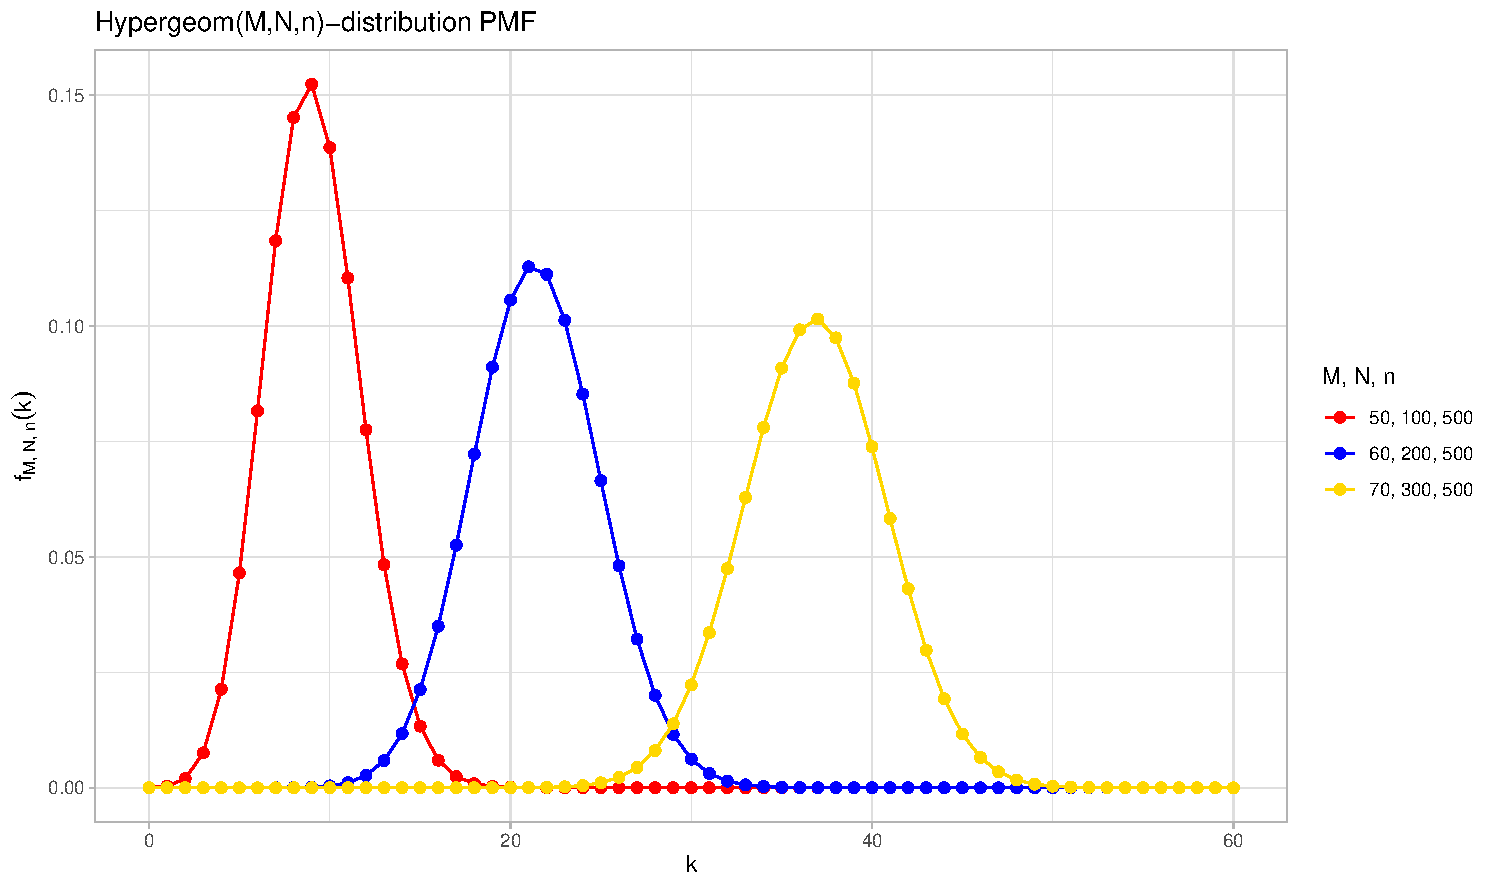
\includegraphics[width=1.0\linewidth]{material/hypergeometric_PMF}
		\label{fig:hypergeometric_PMF}
		&
		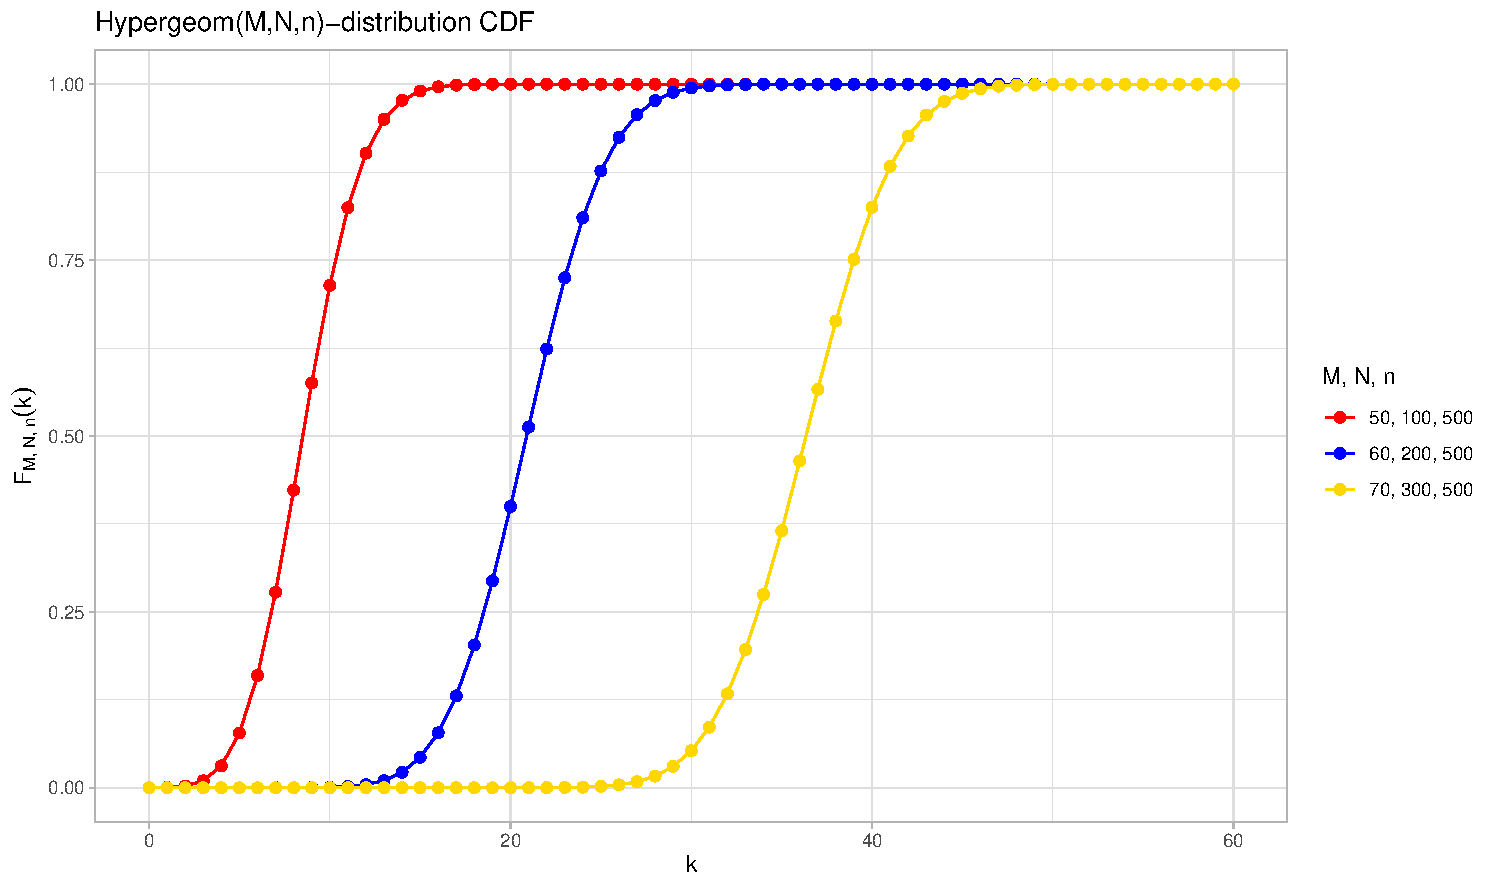
\includegraphics[width=1.0\linewidth]{material/hypergeometric_CDF}
		\label{fig:hypergeometric_CDF}
		\\
		\hline
		Mean
		\[ E\left [ K \right ] = n\dfrac{M}{N} \]
		& Variance
		\[ \text{Var}\left( K\right) = n\dfrac{M}{N}\left( 1-\dfrac{M}{N}\right) \frac{N-n}{N-1} \]
		\\
		\hline
	\end{tabular}
	
	\newpage
	
	\subsection{Binomial($n$,$p$) distribution}
	\begin{tabular}{|*2{>{\centering\arraybackslash}p{.48\textwidth}|}}
		\hline
		Mass function 
		\[ f\left ( k \right ) = \binom{n}{k} p^{k}\left ( 1-p \right )^{n-k} \] 
		& Distribution function
		\[ P\left ( \left \{ K\leq k \right \} \right ) = \sum_{i=0}^{\left \lfloor k \right \rfloor} \binom{n}{i} p^{i} \left ( 1-p \right )^{n-i} \]
		\\
		$\supp f\left( k\right) = \left\lbrace 0,..,n\right\rbrace $ &
		\\
		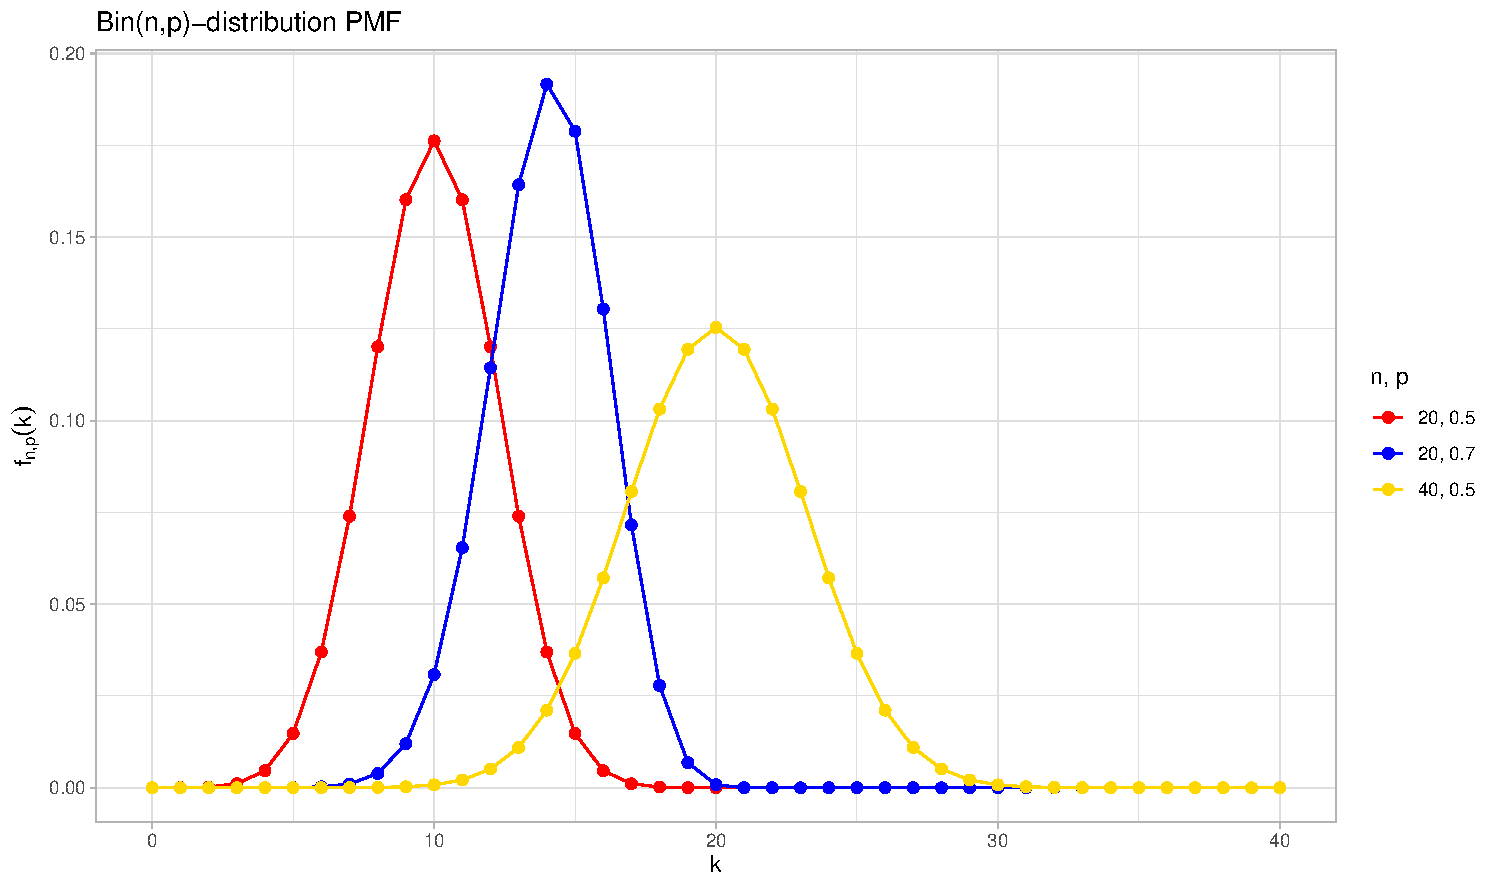
\includegraphics[width=1.0\linewidth]{material/binomial_PMF}
		\label{fig:binomial_PMF}
		&
		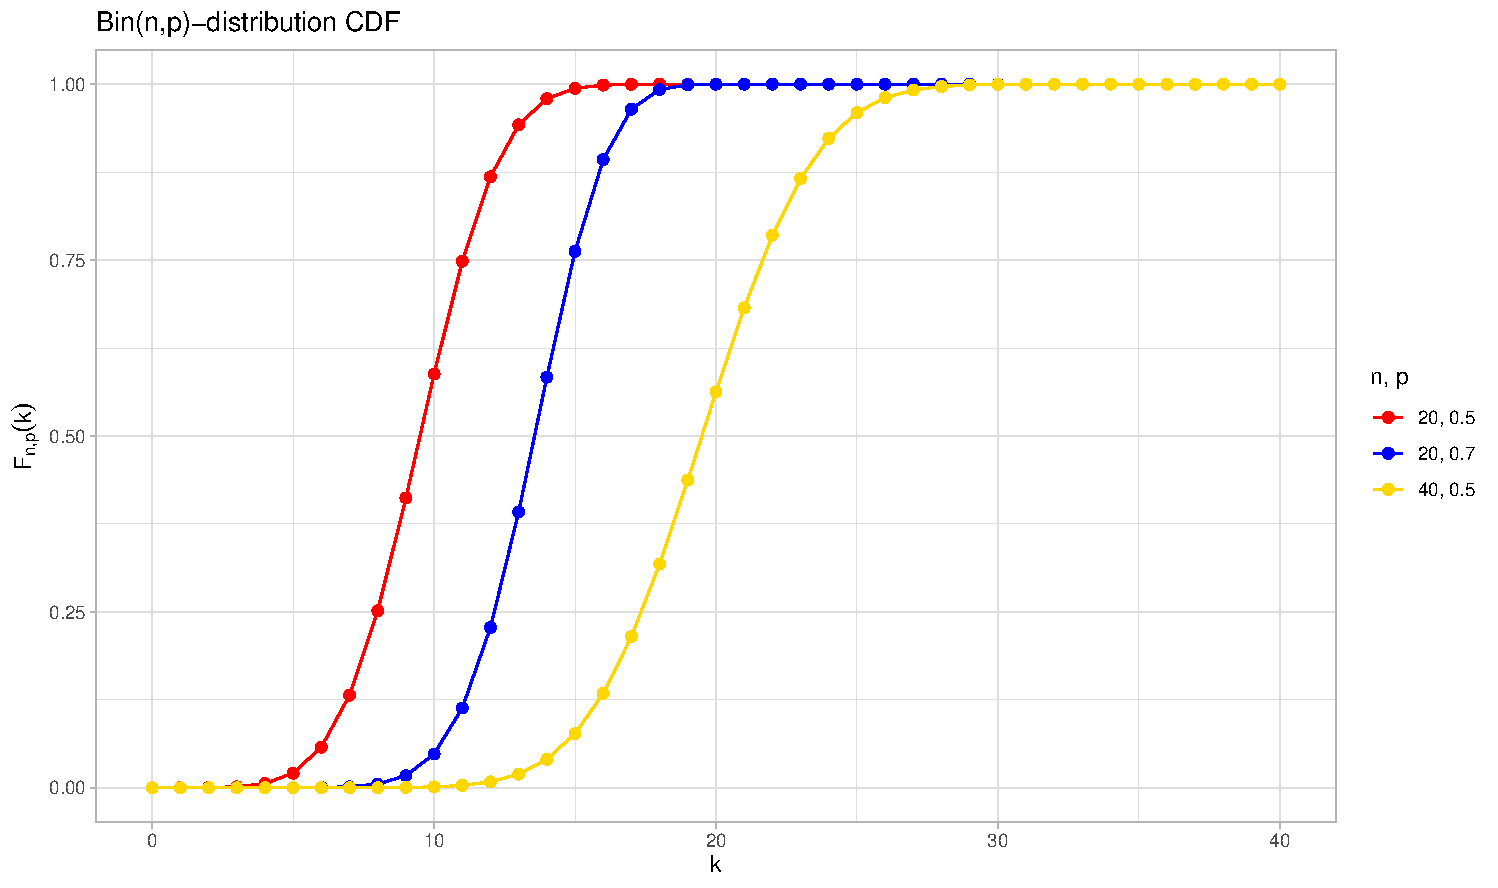
\includegraphics[width=1.0\linewidth]{material/binomial_CDF}
		\label{fig:binomial_CDF}
		\\
	\end{tabular} \\
	
	\vspace{-24pt}
	\begin{center}
		\begin{tabular}{|*3{>{\centering\arraybackslash}p{.3112\textwidth}|}}
			\hline
			Mean
			\[ E\left [ K \right ] = np \]
			& Variance
			\[ \text{Var}\left( K\right) = np \left( 1-p\right) \]
			&Fisher Information
			\[\mathcal{I} \left ( \theta \right ) = \frac{n}{\theta\left ( 1 - \theta \right )} \text{ for fixed } n \]
			\\
		\end{tabular} \\
	\end{center}
	
	\vspace{-22.5pt}
	\begin{center}
		\begin{tabular}{|*2{>{\centering\arraybackslash}p{.48\textwidth}|}}
			\hline
			Moment-generating function
			\[ M_{X}\left( t\right) = \left(1-p+p\exp\left( t\right)  \right) ^{n} \]
			& Characteristic function
			\[ \varphi_{X}\left( t\right) = \left(1-p+p\exp\left( it\right)  \right) ^{n} \]
			\\
			\hline
		\end{tabular} \\
	\end{center}
	
	\vspace{-22.5pt}
	\begin{center}
		\begin{tabular}{|*1{>{\centering\arraybackslash}p{.9865\textwidth}|}}
			\hline
			Maximum Likelihood Estimator
			\[ \hat{p} = \frac{1}{n}\sum_{i=1}^{n}k_{i} \]
			\\
			\hline
		\end{tabular} \\
	\end{center}
	
	\begin{itemize}
		\item $Bin \left( m,p\right) + Bin \left( n,p\right) = Bin \left( m+n,p\right)$ \footnote{Where e.g. $Bin(n,p)$ represents a random variable with $Bin(n,p)$-distribution, not the distribution itself.} \\
	\end{itemize}
	
	\newpage
	
	\subsection{Geometric($p$) distribution}
	\begin{tabular}{|*2{>{\centering\arraybackslash}p{.48\textwidth}|}}
		\hline
		Mass function 
		\[ f\left ( k \right ) = p\left( 1-p\right)^{k-1} \] 
		& Distribution function
		\[ P\left ( \left \{ K \leq k \right \} \right ) = 1-\left( 1-p\right)^{\left \lfloor k \right \rfloor} \]
		\\
		$\supp f\left( k\right) = \mathbb{N}$ &
		\\
		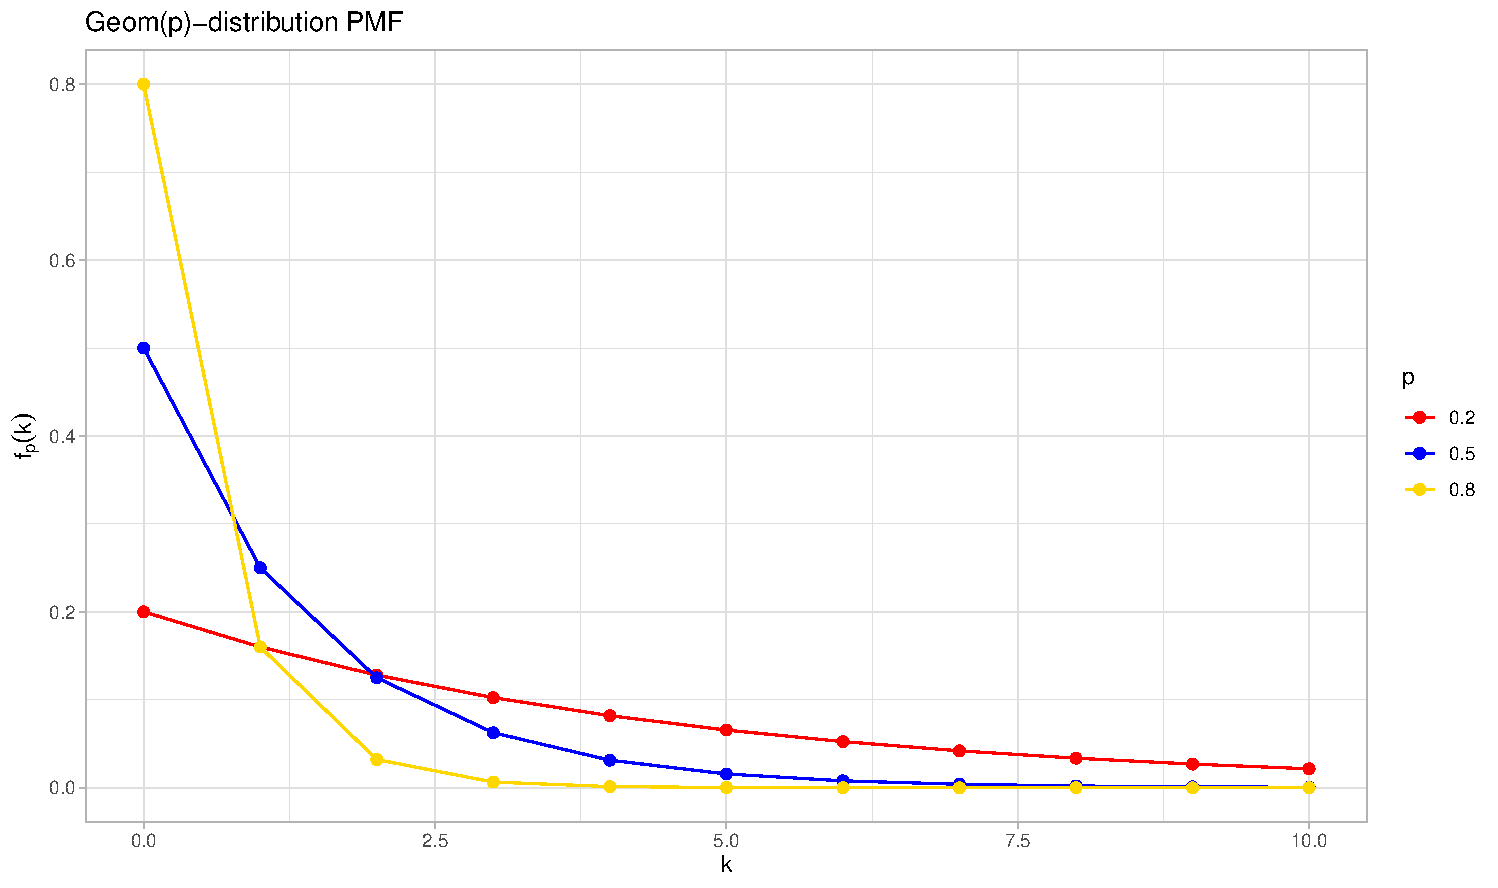
\includegraphics[width=1.0\linewidth]{material/geometric_PMF}
		\label{fig:geometric_PMF}
		&
		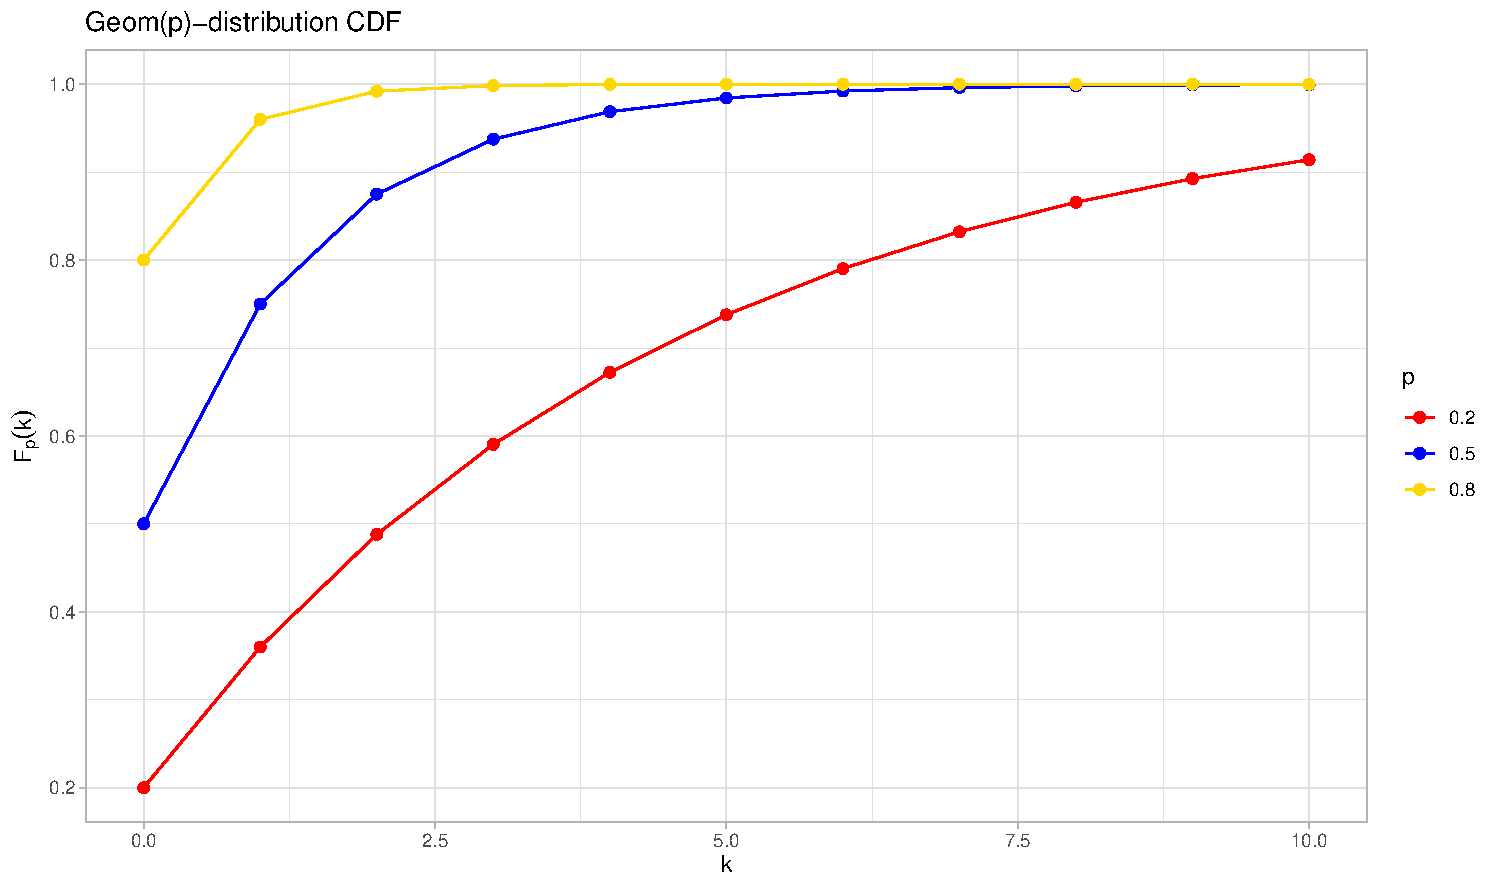
\includegraphics[width=1.0\linewidth]{material/geometric_CDF}
		\label{fig:geometric_CDF}
		\\
	\end{tabular} \\
	
	\vspace{-24pt}
	\begin{center}
		\begin{tabular}{|*3{>{\centering\arraybackslash}p{.3112\textwidth}|}}
			\hline
			Mean
			\[ E\left [ K \right ] = \frac{1}{p} \]
			& Variance
			\[ \text{Var}\left( K\right) = \frac{1}{p^{2}} - \frac{1}{p} \]
			&Fisher Information
			\[ \mathcal{I} \left ( \theta \right ) = \frac{1}{\theta^2}+\frac{1}{\left( 1-\theta\right)^{2} \theta} \]
			\\
		\end{tabular} \\
	\end{center}
	
	\vspace{-22.5pt}
	\begin{center}
		\begin{tabular}{|*2{>{\centering\arraybackslash}p{.48\textwidth}|}}
			\hline
			Moment-generating function
			\[ M_{X}\left( t\right) = \frac{p\exp\left( t\right) }{1-\left( 1-p\right) \exp\left( t\right) } \]
			& Characteristic function
			\[ \varphi_{X}\left( t\right) = \frac{p\exp\left( it\right) }{1-\left( 1-p\right) \exp\left( it\right) } \]
			\\
			\hline
		\end{tabular} \\
	\end{center}
	
	\vspace{-22.5pt}
	\begin{center}
		\begin{tabular}{|*1{>{\centering\arraybackslash}p{.9865\textwidth}|}}
			\hline
			Maximum Likelihood Estimator
			\[ \hat{p} = \frac{n}{\sum_{i=1}^{n}k_{i}} \]
			\\
			\hline
		\end{tabular} \\
	\end{center}
	
	\begin{itemize}
		\item $P\left ( K\geq k+t \mid  K\geq k \right ) = P\left ( K\geq t \right )$ (Memorylessness)
	\end{itemize}
	
	\newpage
	\subsection{Poisson($\lambda$) distribution}
	\begin{tabular}{|*2{>{\centering\arraybackslash}p{.48\textwidth}|}}
		\hline
		Mass function 
		\[ f\left ( k \right ) = \frac{\lambda^{k}}{k!}\exp\left( - \lambda\right) \] 
		& Distribution function
		\[ P\left ( \left \{ K \leq k \right \} \right ) = \sum_{i=0}^{\left \lfloor k \right \rfloor} \frac{\lambda^{i}}{i!} \exp \left( - \lambda\right) \]
		\\
		$\supp f\left( k\right) = \mathbb{N}_{0}$ &
		\\
		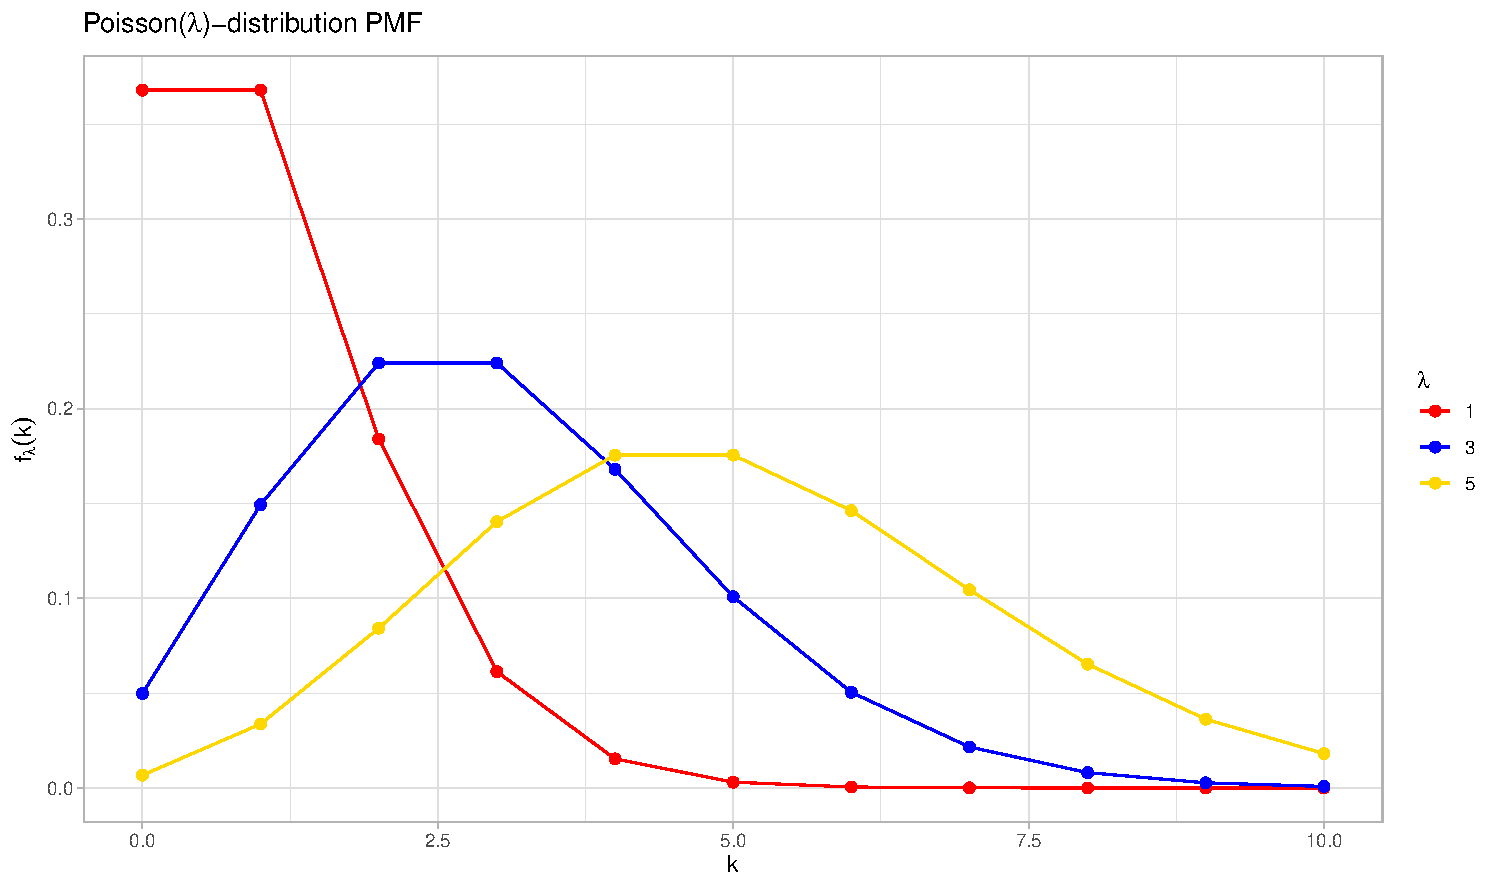
\includegraphics[width=1.0\linewidth]{material/poisson_PMF}
		\label{fig:poisson_PMF}
		&
		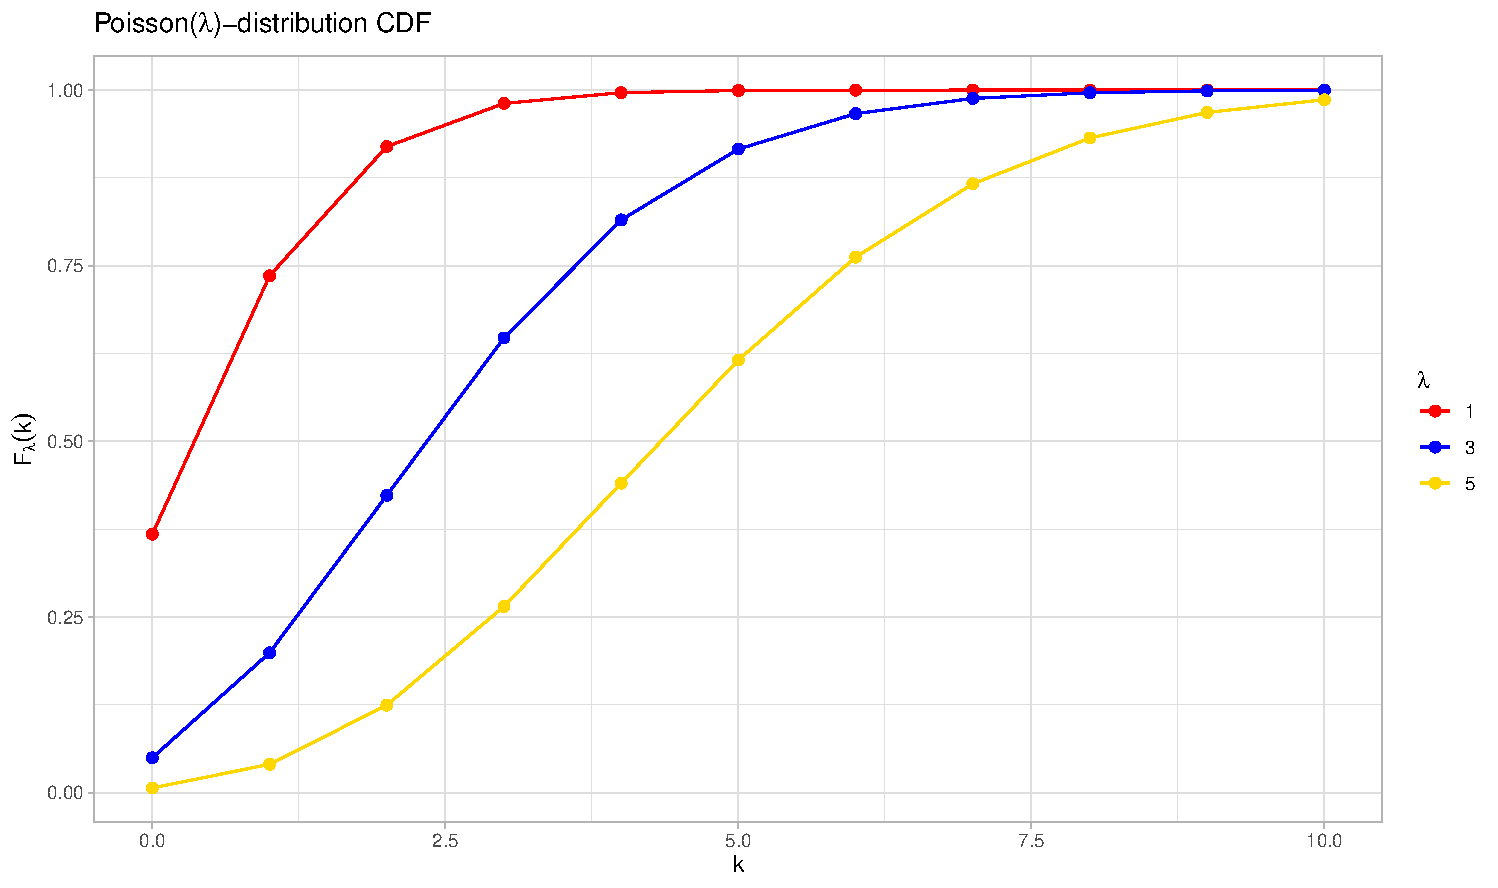
\includegraphics[width=1.0\linewidth]{material/poisson_CDF}
		\label{fig:poisson_CDF}
		\\
	\end{tabular} \\
	
	\vspace{-24pt}
	\begin{center}
		\begin{tabular}{|*3{>{\centering\arraybackslash}p{.3112\textwidth}|}}
			\hline
			Mean
			\[ E\left [ K \right ] = \lambda \]
			& Variance
			\[ \text{Var}\left( K\right) = \lambda \]
			&Fisher Information
			\[ \mathcal{I} \left ( \theta \right ) = \frac{1}{\theta} \]
			\\
		\end{tabular} \\
	\end{center}
	
	\vspace{-22.5pt}
	\begin{center}
		\begin{tabular}{|*2{>{\centering\arraybackslash}p{.48\textwidth}|}}
			\hline
			Moment-generating function
			\[ M_{X}\left( t\right) = \exp\left(\lambda \exp\left(t \right)-1 \right) \]
			& Characteristic function
			\[ \varphi_{X}\left( t\right) = \exp\left(\lambda \exp\left(it \right)-1 \right)  \]
			\\
			\hline
		\end{tabular} \\
	\end{center}
	
	\vspace{-22.5pt}
	\begin{center}
		\begin{tabular}{|*1{>{\centering\arraybackslash}p{.9865\textwidth}|}}
			\hline
			Maximum Likelihood Estimator
			\[ \hat\lambda = \frac{1}{n}\sum_{i=1}^{n}k_{i} \]
			\\
			\hline
		\end{tabular} \\
	\end{center}
	
	\begin{itemize}
		\item $P\left( \alpha\right) + P\left( \beta\right) = P\left( \alpha+\beta\right)$
		\item $Bin\left( n,p\right) = P\left( np\right) \text{ as } n \rightarrow \infty \text{, } p \rightarrow 0$
	\end{itemize}
	
	\newpage
	
	\section{Continous distributions}
	\subsection{Continous uniform($a$,$b$) distribution}
	\begin{tabular}{|*2{>{\centering\arraybackslash}p{.48\textwidth}|}}
		\hline
		Density
		\[ f \left ( x \right ) = \left \{\begin{matrix}
			\frac{1}{b-a} & \text{ for } k \in \left[ a,b\right] \\ 
			0 & \text{otherwise}
		\end{matrix}\right. \] 
		& Distribution function
		\[ F\left ( x \right ) = \left\{\begin{matrix}
			0 & \text{ for } x\leq a\\ 
			\frac{x-a}{b-a} & \text{ for } a< x\leq b\\ 
			1 & \text{ for } x> b
		\end{matrix}\right. \]
		\\
		$\supp f\left( x\right) = \left[ a,b\right] $ &
		\\
		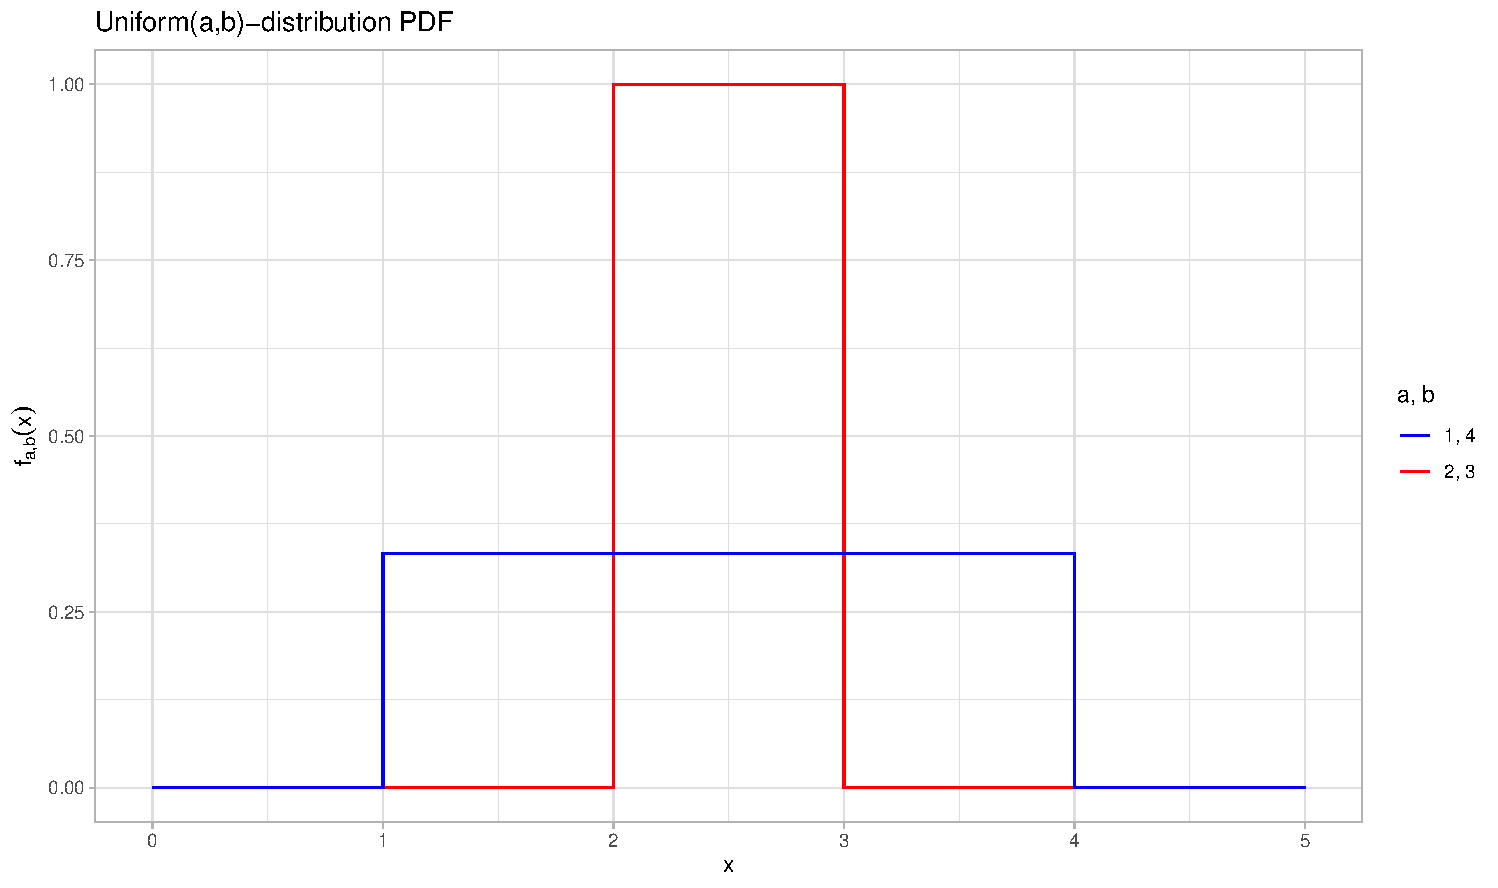
\includegraphics[width=1.0\linewidth]{material/uniform_PDF}
		\label{fig:uniform_PDF}
		&
		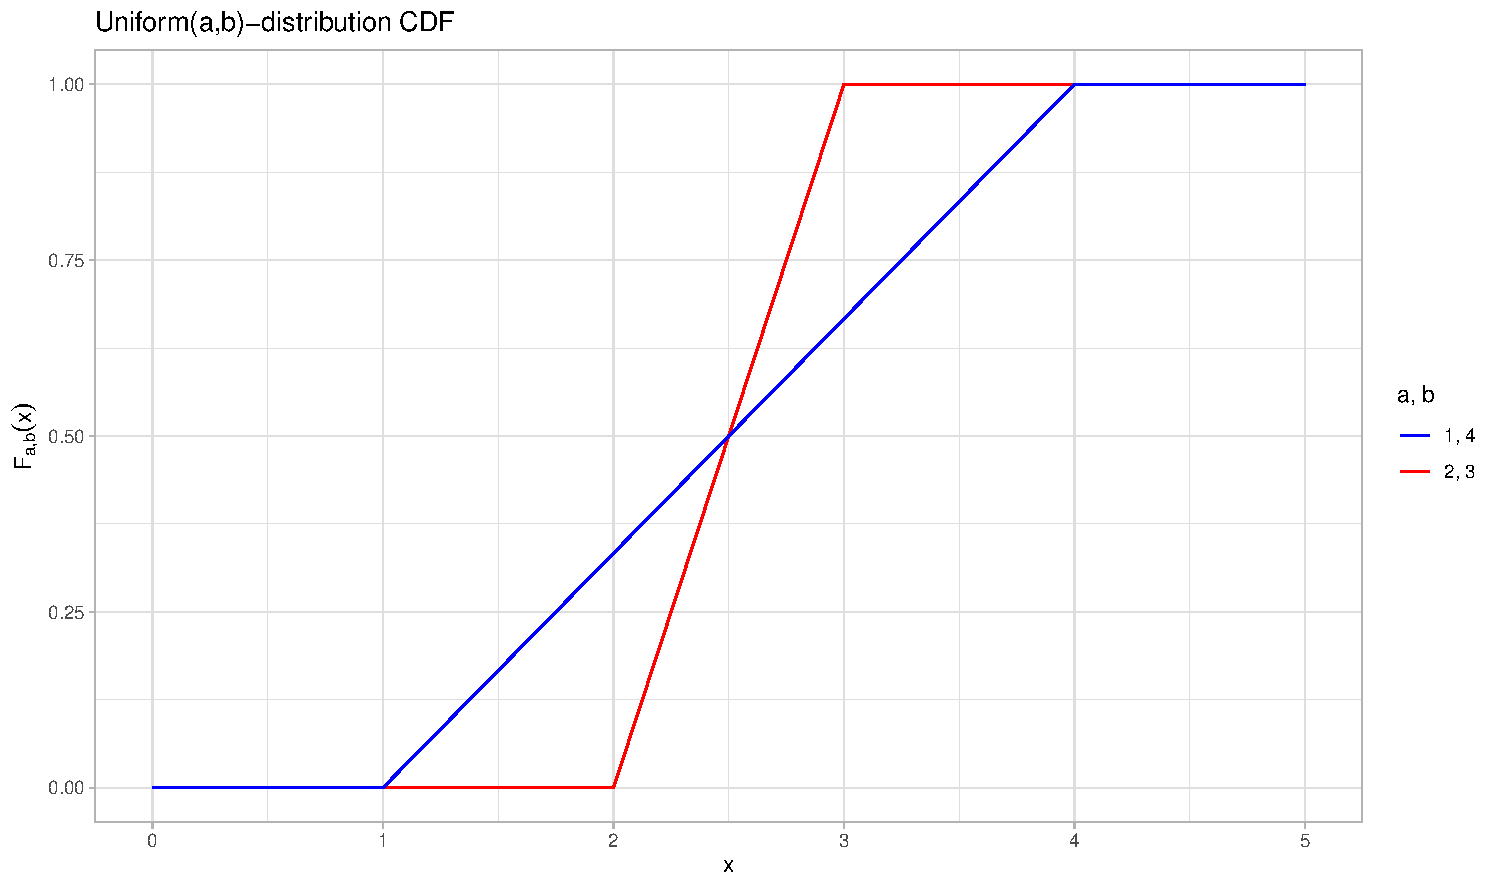
\includegraphics[width=1.0\linewidth]{material/uniform_CDF}
		\label{fig:uniform_CDF}
		\\
		\hline
		Mean
		\[ E\left [ X \right ] = \frac{1}{2} \left( a+b\right) \]
		& Variance
		\[ \text{Var}\left( X\right) = \frac{1}{12} \left( b-a\right)^{2} \]
		\\
	\end{tabular} \\
	
	\vspace{-24pt}
	\begin{center}
		\begin{tabular}{|*2{>{\centering\arraybackslash}p{.48\textwidth}|}}
			\hline
			Moment-generating function
			\[ M_{X}\left( t\right) = \frac{\exp\left(tb \right)-1 }{tb} \text{ for } a=0 \]
			& Characteristic function
			\[ \varphi_{X}\left( t\right) = \frac{\exp\left(itb \right)-1 }{itb} \text{ for } a=0 \]
			\\
		\end{tabular} \\
	\end{center}
	
	\vspace{-22.5pt}
	\begin{center}
		\begin{tabular}{|*1{>{\centering\arraybackslash}p{.9865\textwidth}|}}
			\hline
			Maximum Likelihood Estimator
			\[ \hat{b} = max\left\lbrace x_{1}, ..., x_{n} \right\rbrace \text{ for } a=0 \]
			\\
			\hline
		\end{tabular} \\
	\end{center}
	
	\newpage
	
	\subsection{Normal($\mu$,$\sigma^{2}$) distribution}
	\begin{tabular}{|*2{>{\centering\arraybackslash}p{.48\textwidth}|}}
		\hline
		Density
		\[ f \left ( x \right ) = \frac{1}{{\sigma \sqrt {2\pi } }} \exp\left ( -\frac{\left ( x-\mu \right )^{2}}{2\sigma^{2}} \right )
		\]
		& Distribution function
		\[ F \left ( x \right )=\frac{1}{{\sigma \sqrt {2\pi } }} \int_{- \infty}^{x}\exp\left ( -\frac{\left ( t-\mu \right )^{2}}{2\sigma^{2}} \right ) dt \]
		\\
		$\supp f\left( x\right) = \mathbb{R}$ &
		\\	
		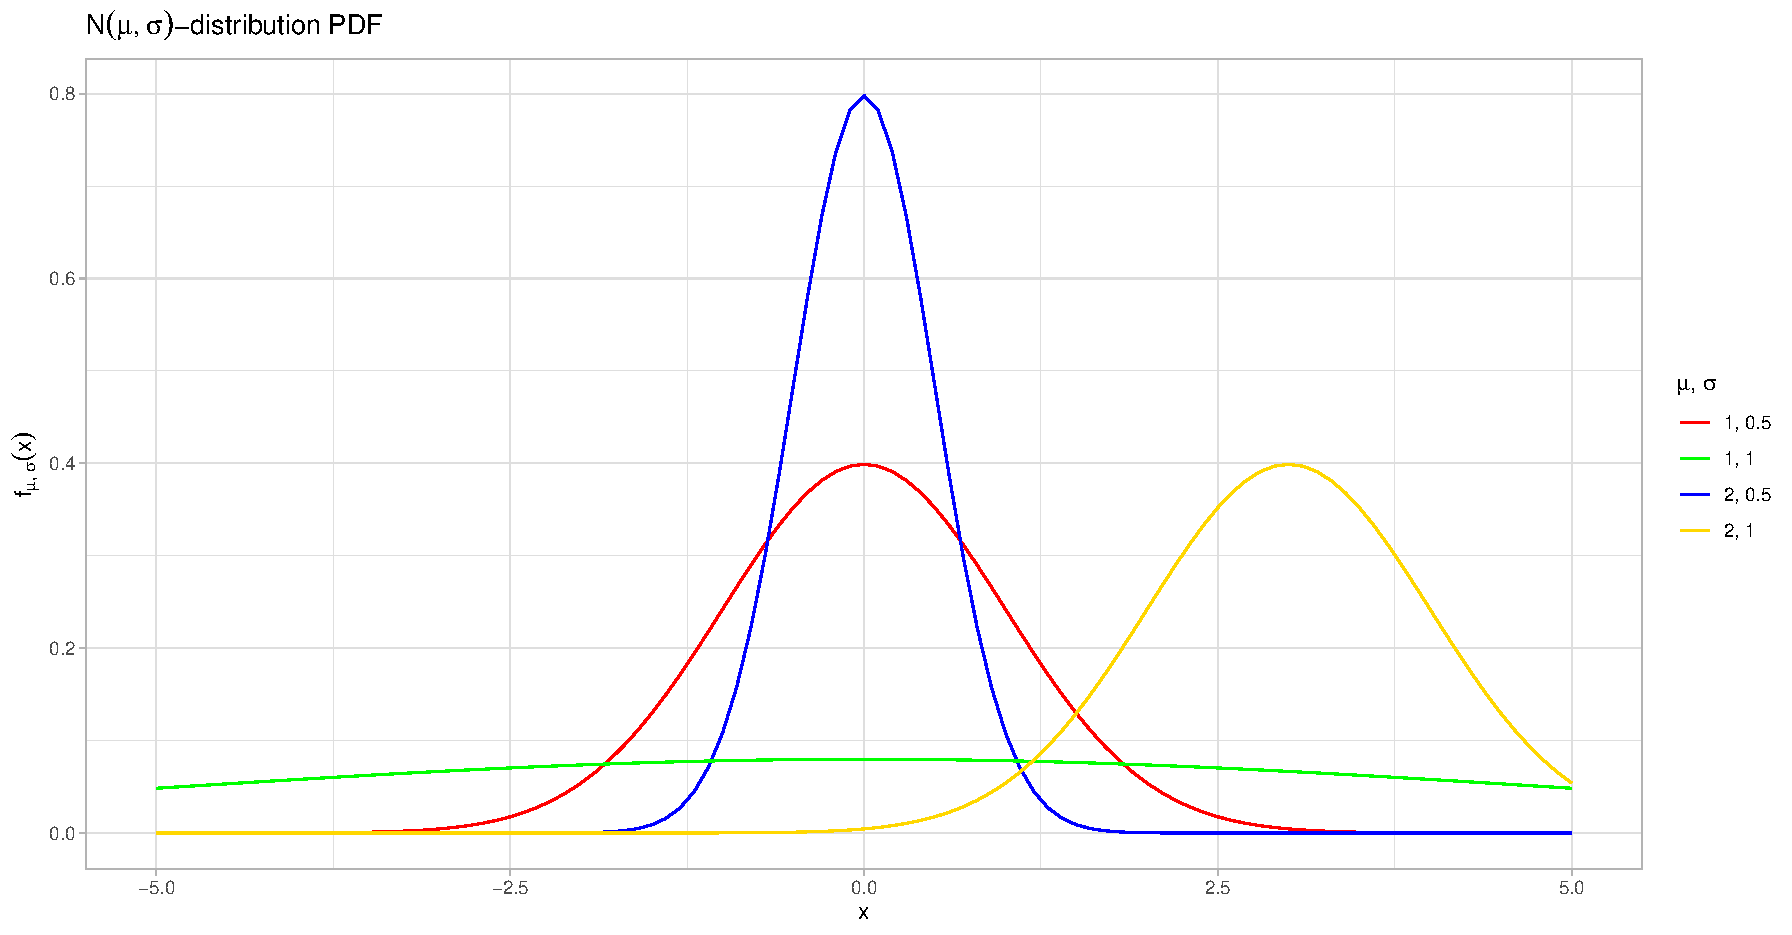
\includegraphics[width=1.0\linewidth]{material/normal_PDF}
		\label{fig:normal_PDF}
		&
		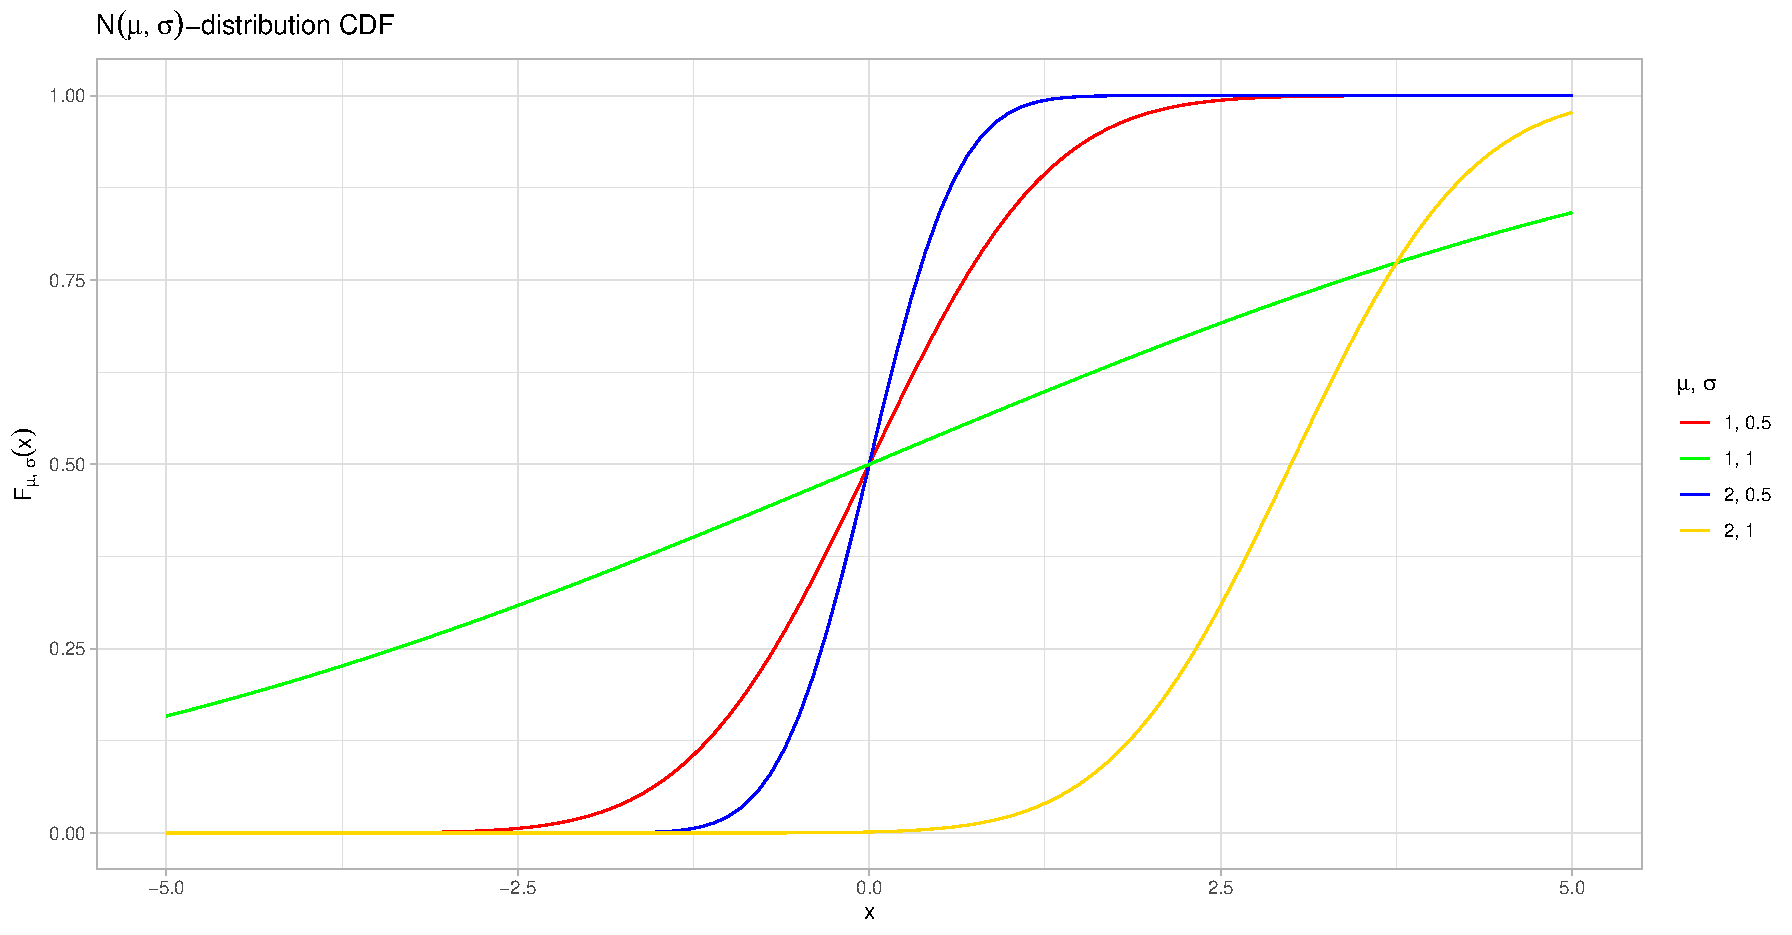
\includegraphics[width=1.0\linewidth]{material/normal_CDF}
		\label{fig:normal_CDF}
		\\
	\end{tabular}\\
	
	\vspace{-24pt}
	\begin{center}
		\begin{tabular}{|*3{>{\centering\arraybackslash}p{.3112\textwidth}|}}
			\hline
			Mean
			\[ E\left [ X \right ] = \mu \]
			& Variance
			\[ \text{Var}\left( X\right) = \sigma^{2} \]
			& Fisher Information
			\[\mathcal{I} \left ( \mu,\sigma^{2} \right ) = 
			\begin{pmatrix}
				\frac{1}{\sigma^{2}} & 0\\ 
				0 & \frac{1}{2\sigma^{4}}
			\end{pmatrix}\]
			\\
		\end{tabular} \\
	\end{center}
	
	\vspace{-22.5pt}
	\begin{center}
		\begin{tabular}{|*2{>{\centering\arraybackslash}p{.48\textwidth}|}}
			\hline
			Moment-generating function
			\[ M_{X}\left( t\right) = \exp\left( t\mu+\frac{1}{2}\sigma_{2}t^{2}\right) \]
			& Characteristic function
			\[ \varphi_{X}\left( t\right) = \exp\left(it\mu+\frac{1}{2}\sigma_{2}t^{2}\right) \]
			\\
			\hline
		\end{tabular} \\
	\end{center}
	
	\vspace{-22.5pt}
	\begin{center}
		\begin{tabular}{|*2{>{\centering\arraybackslash}p{.48\textwidth}|}}
			\hline
			\begin{tabular}{ c|c }
				Order & Raw moment \\
				\hline
				2 & $\mu^{2}+\sigma_{2}$ \\
				3 & $\mu_{3}+3\mu\sigma_{2}$ \\
				4 & $\mu_{4}+6\mu_{2}\sigma_{2}+3\mu_{4}$ \\
				5 & $\mu_{5}+10\mu_{3}\sigma_{2}+15\mu\sigma_{4}$
			\end{tabular}
			& \vspace{-30pt}
			Maximum Likelihood Estimator
			\[ \hat\mu = \frac{1}{n}\sum_{i=1}^{n}x_{i} \hspace{25pt} \hat\sigma^{2} = \frac{1}{n}\sum_{i=1}^{n}\left ( x_{i} - \bar{x_{n}} \right )^{2} \]
			\\
			\hline
		\end{tabular} \\
	\end{center}
	
	\vspace{-22.5pt}
	\begin{center}
		\begin{tabular}{|*1{>{\centering\arraybackslash}p{.9865\textwidth}|}}
			Confidence intervals with confidence level $\left( 1-\alpha\right)$
			\[\mu \in \left [ \hat{\mu} - \tau_{n-1}\left ( 1-\frac{\alpha}{2} \right )\sqrt {\frac{\hat{\sigma}^{2}}{n}}, \hat{\mu} + \tau_{n-1}\left ( 1-\frac{\alpha}{2} \right )\sqrt {\frac{\hat{\sigma}^{2}}{n}} \right ] \hspace{10pt} \sigma^{2} \in \left [ \frac{\left ( n-1 \right )\hat{\sigma}^{2}}{\chi^{2}_{n-1}\left ( 1-\frac{\alpha}{2} \right )} , \frac{\left ( n-1 \right )\hat{\sigma}^{2}}{\chi^{2}_{n-1}\left (\frac{\alpha}{2} \right )}\right ] \]
			\\
			\hline
		\end{tabular} \\
	\end{center}
	
	\begin{itemize}
		\item $N\left( \mu_{1},\sigma_{1}^{2}\right) + N\left( \mu_{2},\sigma_{2}^{2}\right) = N\left( \mu_{1}+\mu_{2},\sigma_{1}^{2}+\sigma_{2}^{2}\right)$
	\end{itemize}
	
	\newpage
	
	\subsection{Gamma($\lambda$,$p$) distribution}
	The Gamma-function $\Gamma:\left( 0,\infty \right) \to \mathbb{R}$ is defined by
	\begin{align*}
		\Gamma\left( x\right) = \int_{0}^{\infty}t^{x-1}\exp\left ( -t \right ) dt.
	\end{align*}
	It has the following useful properties
	\begin{itemize}
		\item $\Gamma\left ( x+1 \right )=x\Gamma\left ( x \right ) \forall x>0$,
		\item $\Gamma\left ( n+1 \right )=n! \forall n\in\mathbb{N}$,
		\item $\Gamma\left ( \frac{1}{2} \right )= \sqrt{\pi}$.
	\end{itemize}
	\vspace{4pt}
	\begin{tabular}{|*2{>{\centering\arraybackslash}p{.48\textwidth}|}}
		\hline
		Density
		\[ f \left ( x \right ) = \frac{\lambda^{p}}{\Gamma\left ( p \right )} x^{p-1} \exp\left ( - \lambda x \right ) 
		\] 
		& Distribution function
		\[ F \left ( x \right ) = \left\{\begin{matrix}
			0 & \text{ for } x\leq 0\\ 
			\frac{\lambda^{p}}{\Gamma\left ( p \right )}\int_{0}^{x} t^{p-1} \exp\left ( - \lambda t \right ) dt  & \text{ for } x>0\\ 
		\end{matrix} \right. \]
		\\
		$\supp f\left( x\right) = \mathbb{R}^{+}_{0}$ &
		\\
		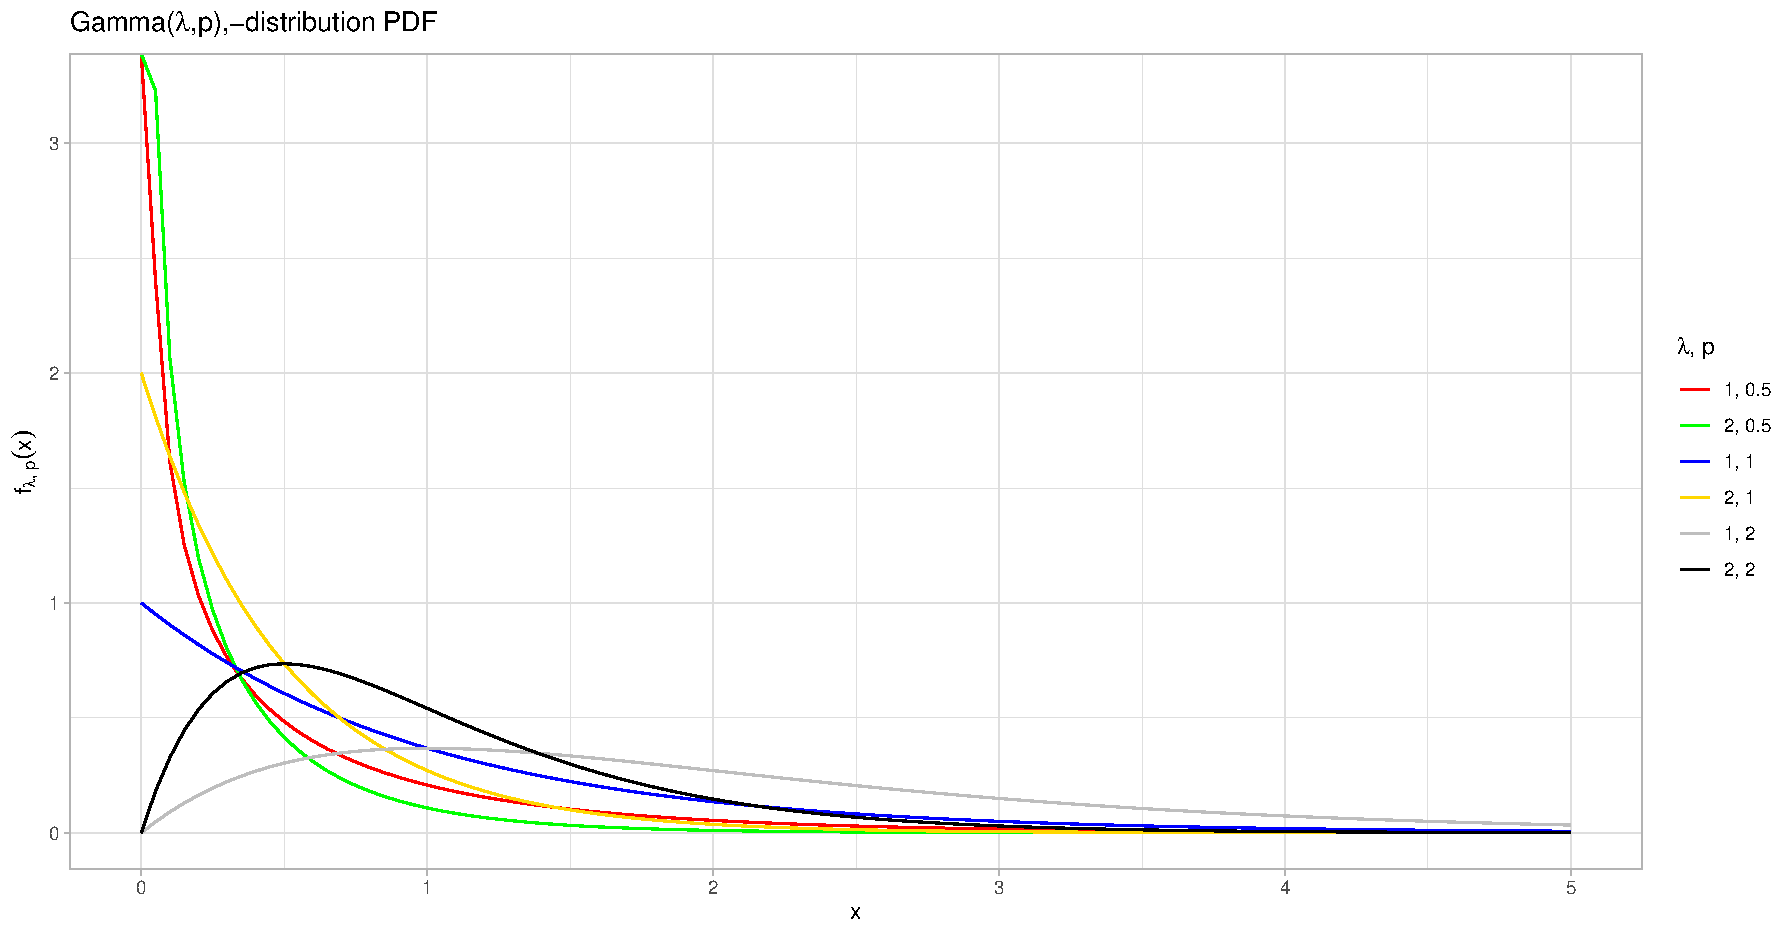
\includegraphics[width=1.0\linewidth]{material/gamma_PDF}
		\label{fig:gamma_PDF}
		&
		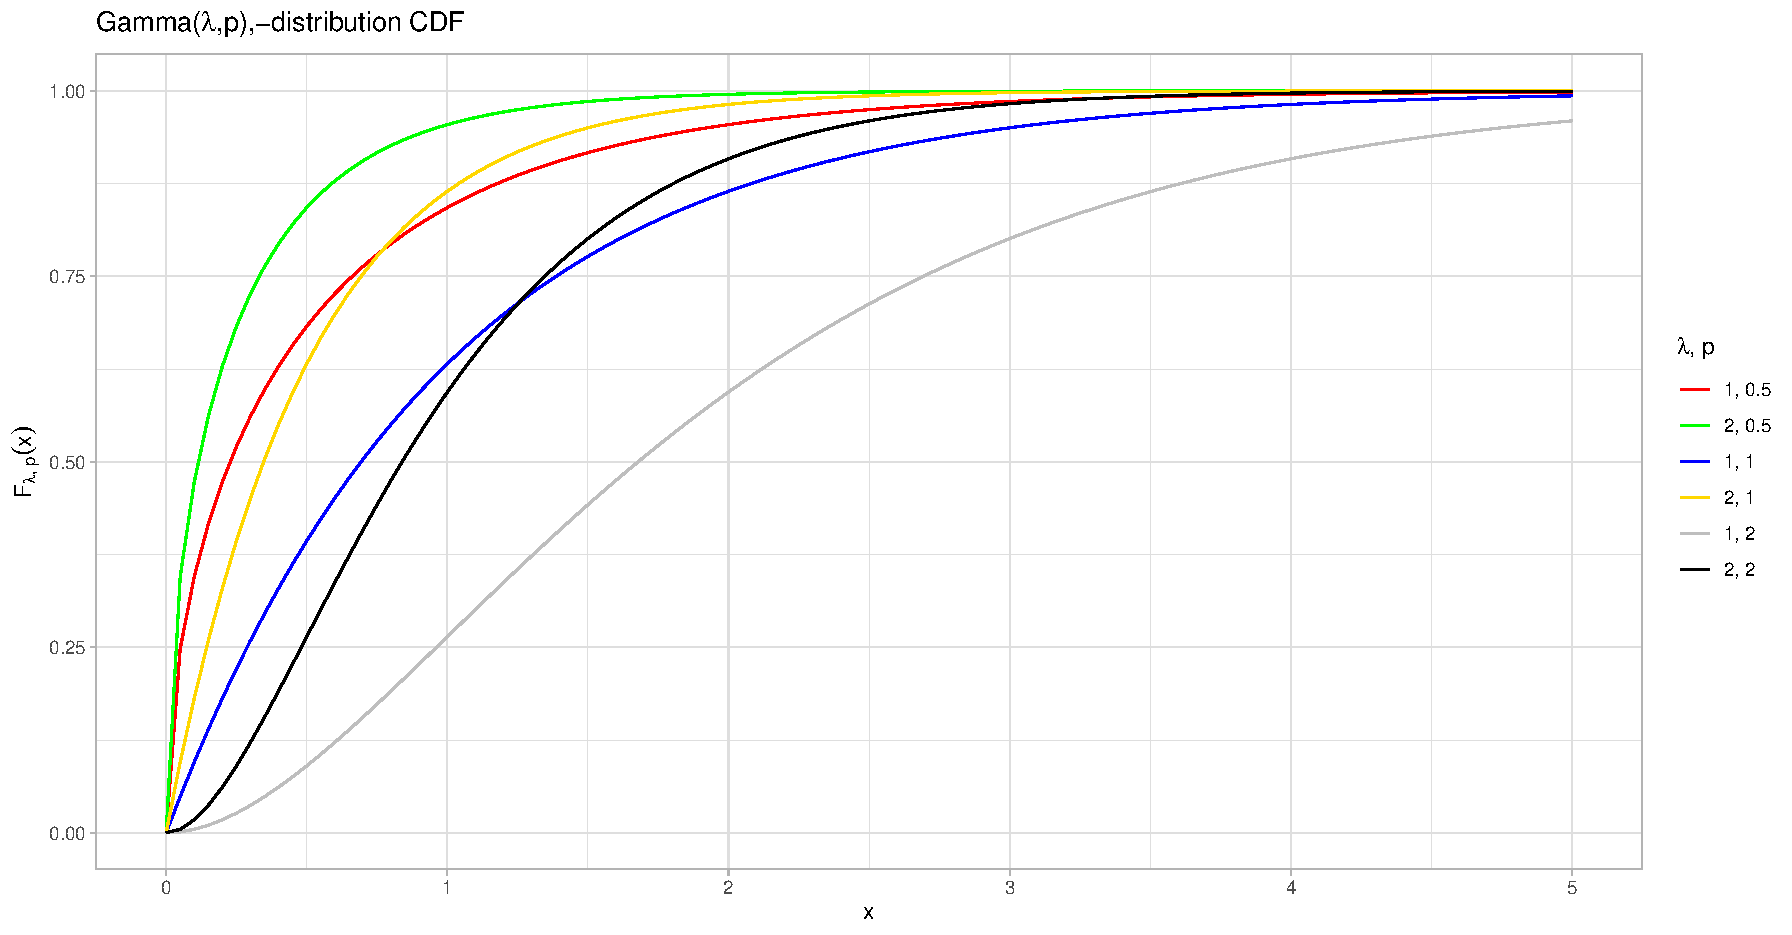
\includegraphics[width=1.0\linewidth]{material/gamma_CDF}
		\label{fig:gamma_CDF}
		\\
	\end{tabular} \\
	
	\vspace{-24pt}
	\begin{center}
		\begin{tabular}{|*3{>{\centering\arraybackslash}p{.3112\textwidth}|}}
			\hline
			Mean
			\[ E\left [ X \right ] = \frac{p}{\lambda} \]
			& Variance
			\[ \text{Var}\left( X\right) = \frac{p}{\lambda^{2}} \]
			&Fisher Information
			\[ \mathcal{I} \left ( \lambda,p \right ) = 
			\begin{pmatrix}
				\frac{d^{2}}{dp^{2}}\log \left(  \Gamma\left( p\right) \right)  & -\frac{1}{\lambda}\\ 
				-\frac{1}{\lambda} & \frac{p}{\lambda^{2}}
			\end{pmatrix} \]
			\\
		\end{tabular} \\
	\end{center}
	
	\vspace{-22.5pt}
	\begin{center}
		\begin{tabular}{|*2{>{\centering\arraybackslash}p{.48\textwidth}|}}
			\hline
			Moment-generating function
			\[ M_{X}\left( t\right) = \left(1-\frac{t}{\lambda} \right) ^{-p} \]
			& Characteristic function
			\[ \varphi_{X}\left( t\right) = \left(1-\frac{it}{\lambda} \right) ^{-p} \]
			\\
			\hline
		\end{tabular} \\
	\end{center}
	
	\vspace{-22.5pt}
	\begin{center}
		\begin{tabular}{|*1{>{\centering\arraybackslash}p{.9865\textwidth}|}}
			\hline
			Maximum Likelihood Estimator
			\[ \hat\lambda = \frac{p}{\sum_{i=1}^{n}x_{i}} \]
			\\
			\hline
		\end{tabular} \\
	\end{center}
	
	\begin{itemize}
		\item $\Gamma \left( \lambda,p\right) + \Gamma \left( \lambda,q\right) = \Gamma \left( \lambda,p+q\right)$
		\item $\Gamma\left( \lambda,1\right) = Exp\left( \lambda\right) $
	\end{itemize}
	
	\newpage
	
	\subsection{Beta($p$,$q$) distribution}
	The Beta-function $B:\left( 0,\infty \right) \times \left( 0,\infty \right) \to \mathbb{R}^{2}$ is defined by
	\begin{align*}
		B\left( q,p\right) = \dfrac{\Gamma\left( q\right) \Gamma\left( p\right) }{\Gamma\left( q+p\right) }.
	\end{align*}
	\begin{tabular}{|*2{>{\centering\arraybackslash}p{.48\textwidth}|}}
		\hline
		Density
		\[ f \left ( x \right ) = \frac{1}{B\left ( p,q \right )}x^{p-1}\left ( 1-x \right )^{q-1}
		\] 
		& Distribution function
		\[ F \left ( x \right ) = \left\{\begin{matrix}
			0 & \text{ for } x<0\\ 
			\frac{1}{B\left ( p,q \right )}\int_{0}^{x}t^{p-1}\left ( 1-t \right )^{q-1} & \text{ for } 0\leq x\leq 1\\ 
			1 & \text{ for } x> 1
		\end{matrix}\right. \]
		\\
		$\supp f\left( x\right) = \left[ 0,1\right] $ &
		\\
		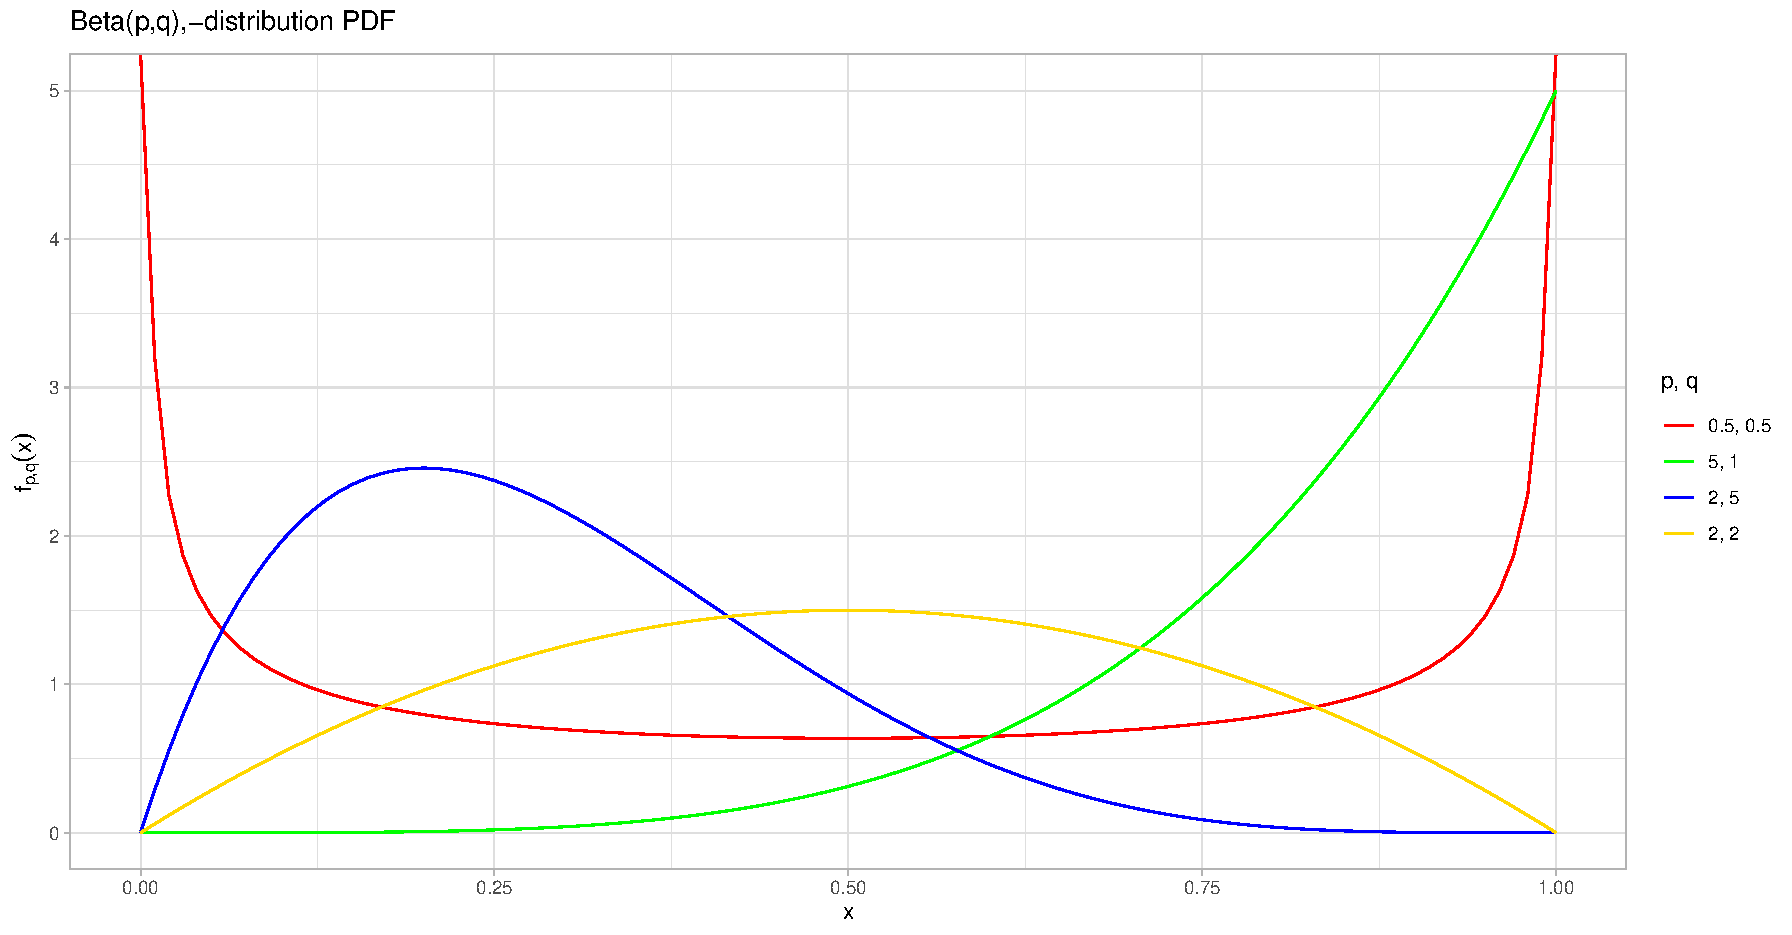
\includegraphics[width=1.0\linewidth]{material/beta_PDF}
		\label{fig:rplot}
		&
		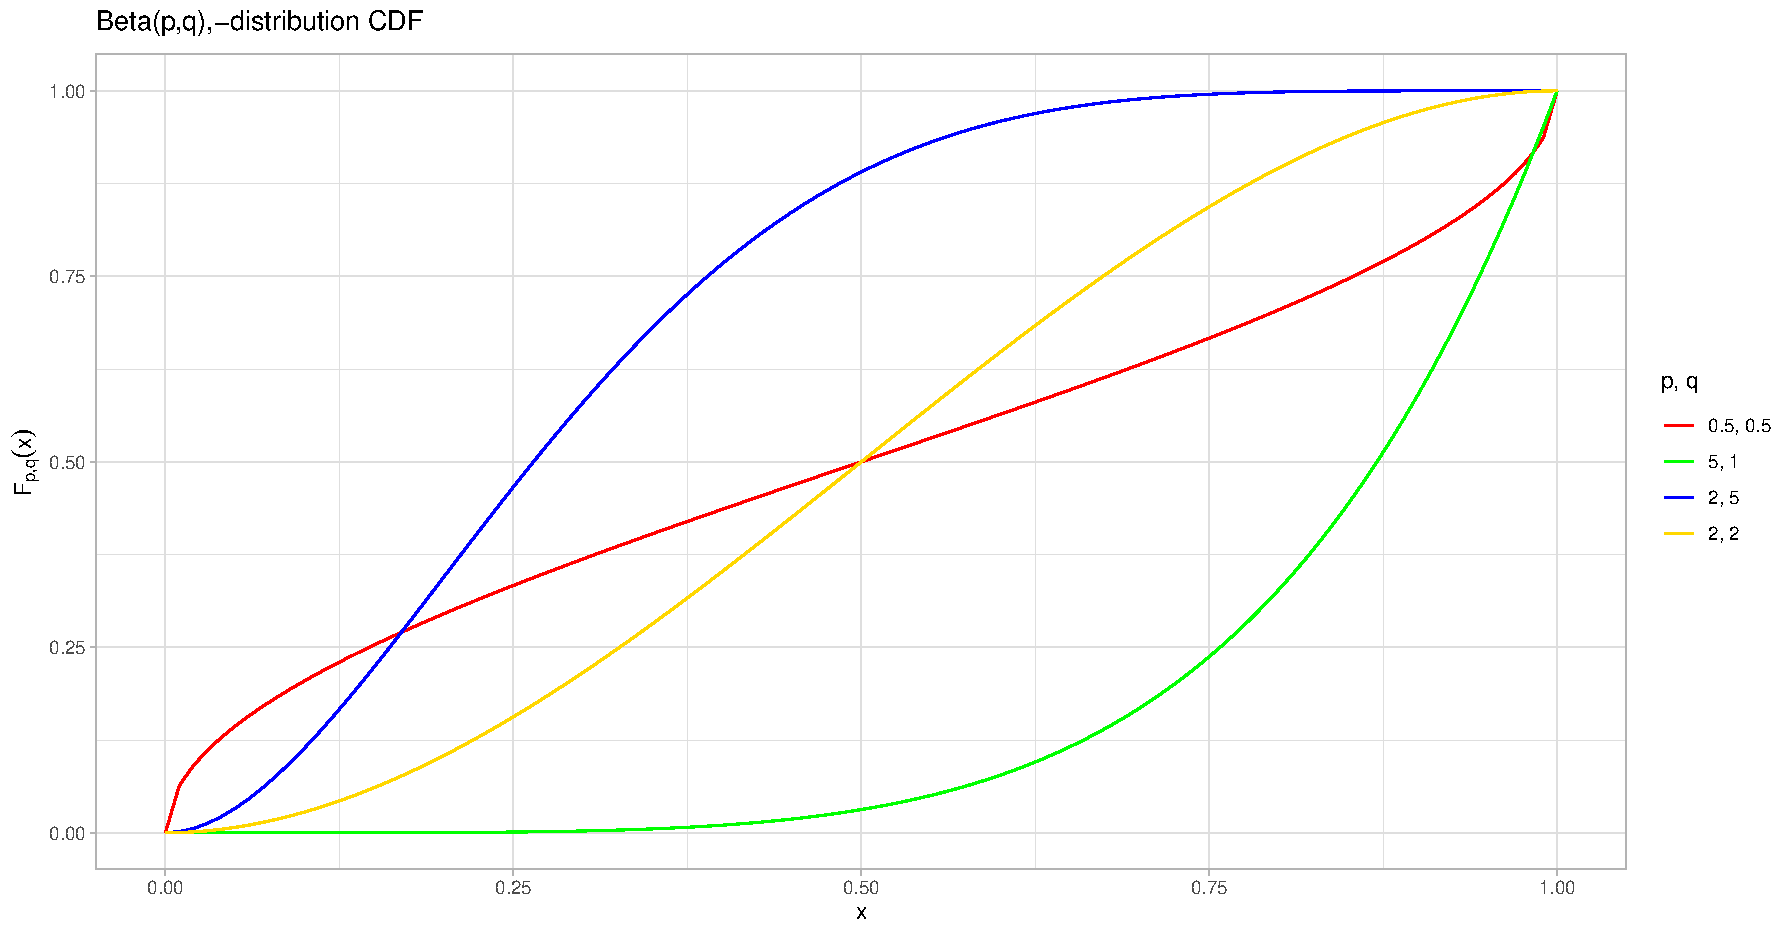
\includegraphics[width=1.0\linewidth]{material/beta_CDF}
		\label{fig:beta_CDF}
		\\
		\hline
		Mean
		\[ E\left [ X \right ] = \frac{p}{p+q} \]
		& Variance
		\[ \text{Var}\left( X\right) = \frac{pq}{\left( p+q+1\right) \left( p+q\right)^{2}} \]
		\\
	\end{tabular} \\
	
	\vspace{-24pt}
	\begin{center}
		\begin{tabular}{|*1{>{\centering\arraybackslash}p{.9865\textwidth}|}}
			\hline
			Fisher Information
			\[ \mathcal{I} \left ( p,q \right ) =  
			\begin{pmatrix}
				\frac{\partial^{2}\log\left ( \Gamma\left ( p \right ) \right )}{\partial p^{2}} - \frac{\partial^{2}\log\left ( \Gamma\left ( p+q \right ) \right )}{\partial \left ( p+q \right )^{2}} & \frac{\partial^{2}\log\left ( \Gamma\left ( q \right ) \right )}{\partial q^{2}} - \frac{\partial^{2}\log\left ( \Gamma\left ( p+q \right ) \right )}{\partial \left ( p+q \right )^{2}}\\ 
				\frac{\partial^{2}\log\left ( \Gamma\left ( q \right ) \right )}{\partial q^{2}} - \frac{\partial^{2}\log\left ( \Gamma\left ( p+q \right ) \right )}{\partial \left ( p+q \right )^{2}} & 
				-\frac{\partial^{2}\log\left ( \Gamma\left ( p+q \right ) \right )}{\partial \left ( p+q \right )^{2}}
			\end{pmatrix} \]
			\\
		\end{tabular} \\
	\end{center}
	
	\vspace{-22.5pt}
	\begin{center}
		\begin{tabular}{|*2{>{\centering\arraybackslash}p{.48\textwidth}|}}
			\hline
			Moment-generating function
			\[ M_{X}\left( t\right) = 1+\sum_{i=1}^{\infty}\left ( \prod_{j=0}^{i-1}\frac{p+j}{p+q+j} \right )\frac{t^{i}}{i!} \]
			& Characteristic function
			\[- \footnotemark[2] \]
			\\
			\hline
		\end{tabular} \\
	\end{center}
	
	\begin{itemize}
		\item $B\left( p,q\right) = \dfrac{\Gamma\left( \lambda, p \right) }{\Gamma\left( \lambda,p\right) + \Gamma\left( \lambda,q\right) }$
	\end{itemize}
	
	\footnotetext[2]{The function has no closed-form expression.}
	
	\newpage
	
	\subsection{Chi-square($n$) distribution}
	\begin{tabular}{|*2{>{\centering\arraybackslash}p{.48\textwidth}|}}
		\hline
		Density
		\[ f \left ( x \right ) = \frac{1}{2^{\frac{n}{2}}\Gamma\left ( \frac{n}{2} \right )} x^{\frac{n}{2}-1} \exp\left ( -\frac{x}{2} \right )
		\] 
		& Distribution function
		\[ F \left ( x \right ) = \left\{\begin{matrix}
			0 & \text{ for } x\leq 0\\ 
			1-\frac{\gamma\left ( \frac{n}{2},\frac{x}{2} \right )}{\Gamma\left ( \frac{n}{2} \right )} & \text{ for } x> 0 
		\end{matrix}\right. \]
		\\
		$\supp f\left( x\right) = \mathbb{R}^{+}_{0}$ &
		\\
		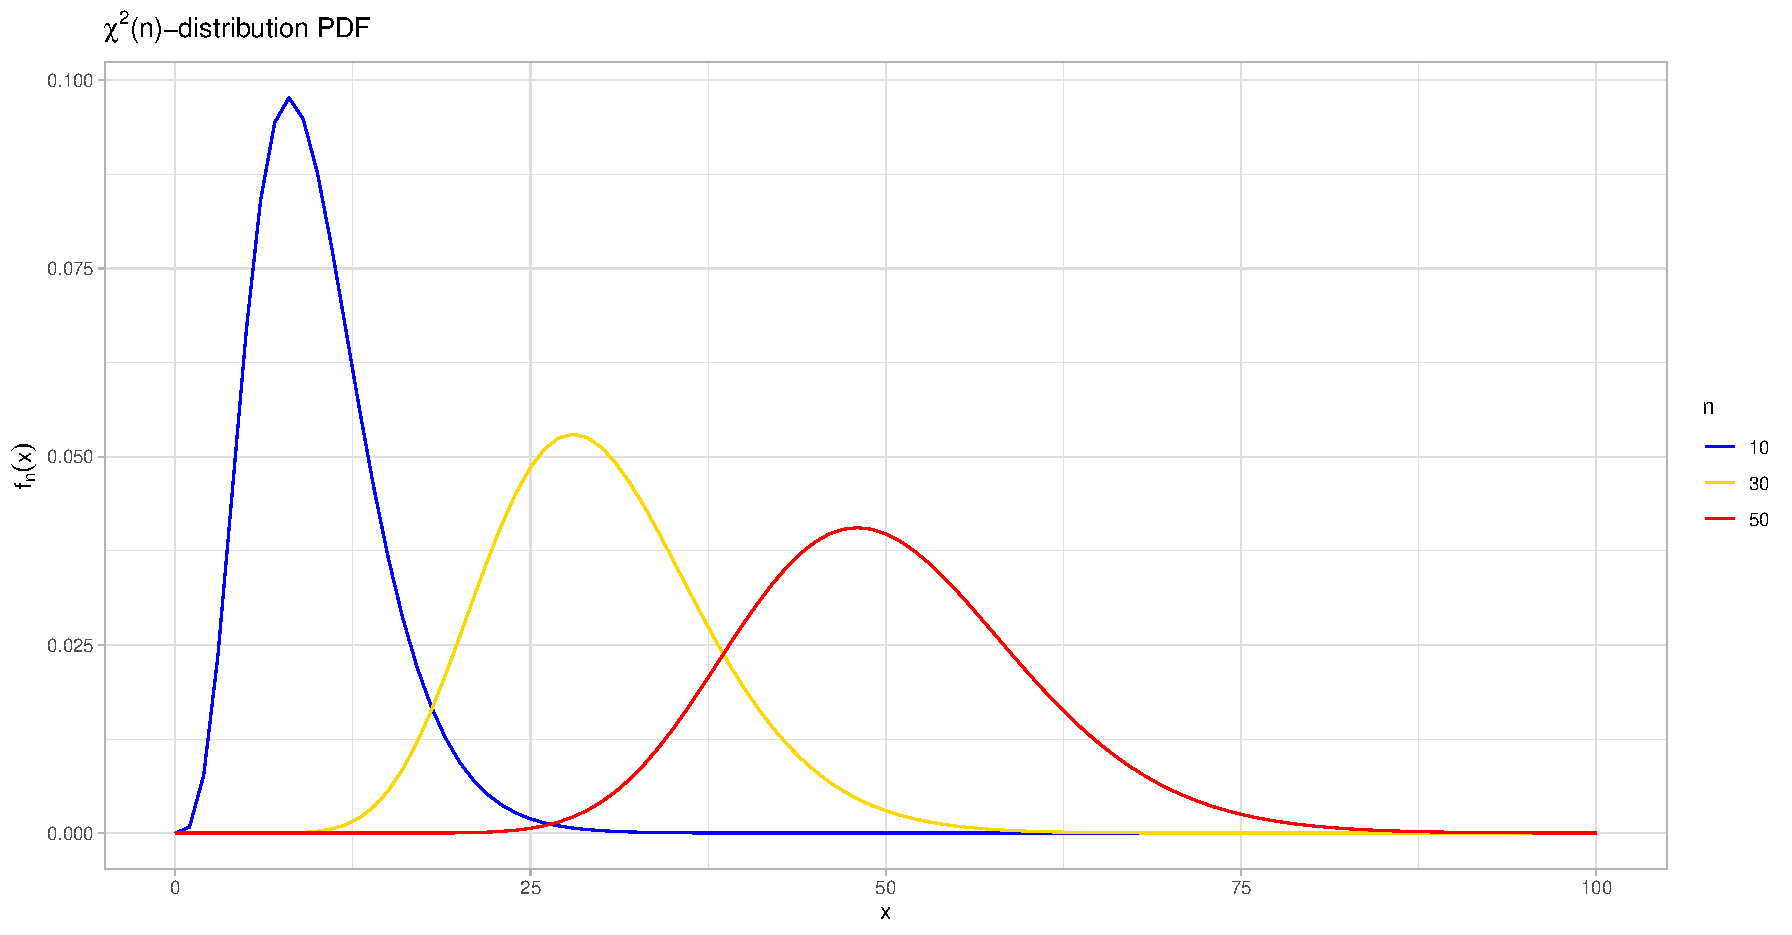
\includegraphics[width=1.0\linewidth]{material/chi_PDF}
		\label{fig:chi_PDF}
		&
		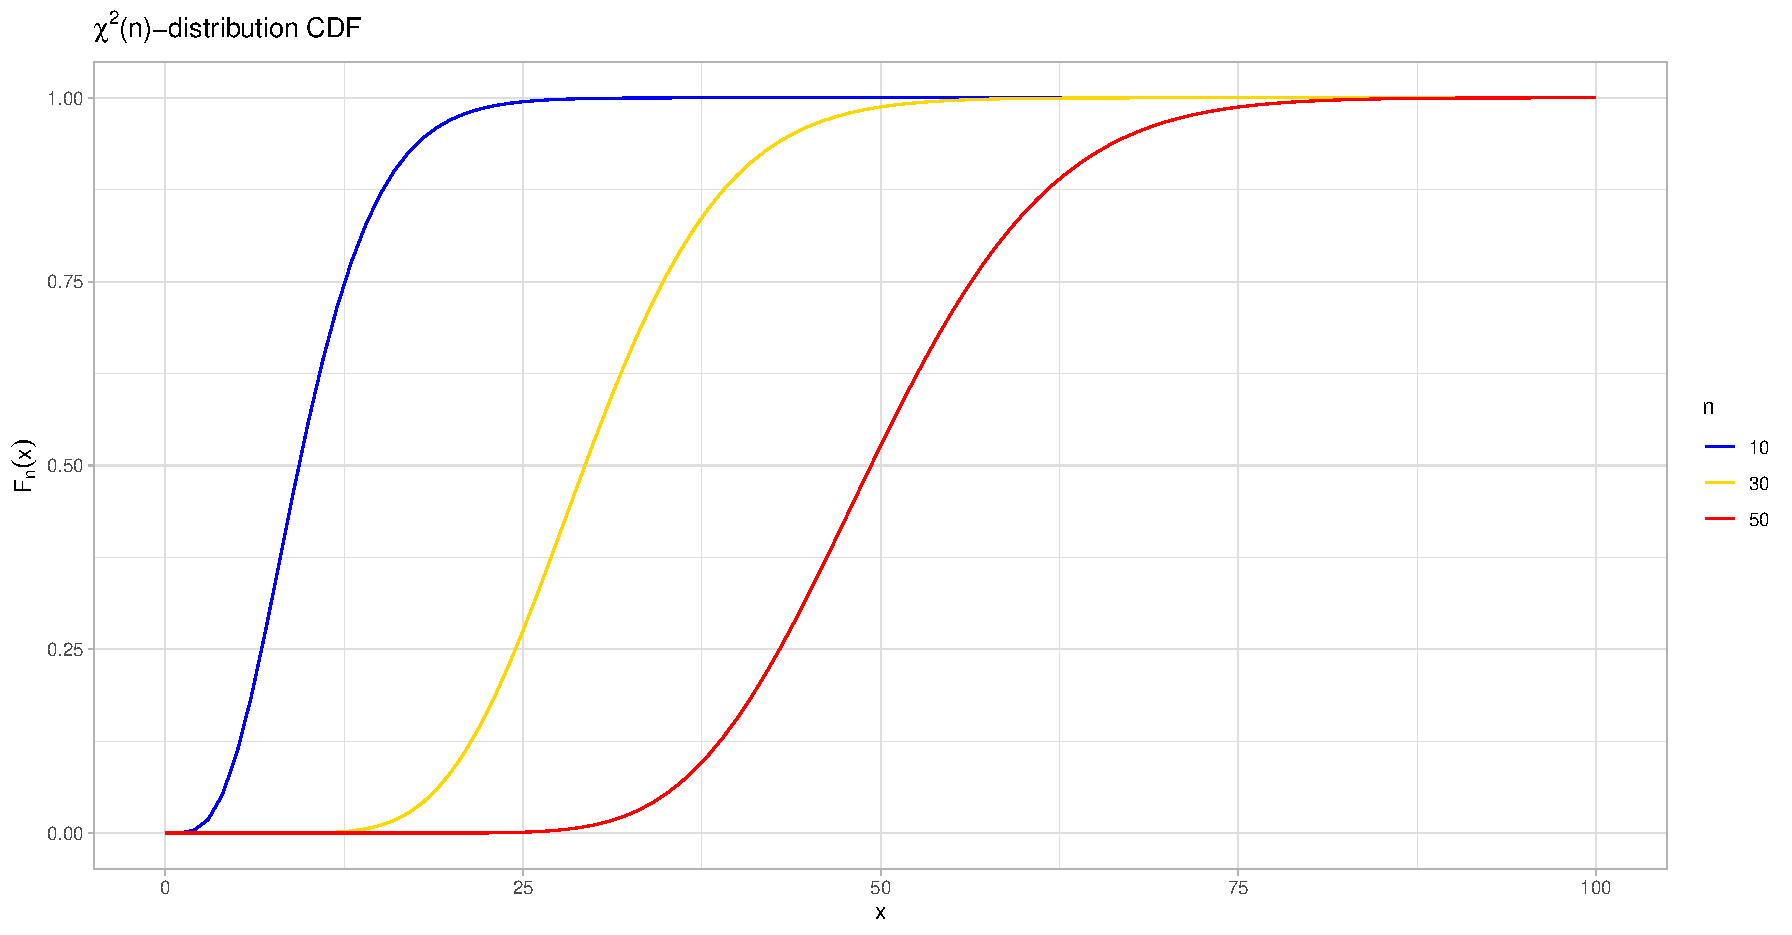
\includegraphics[width=1.0\linewidth]{material/chi_CDF}
		\label{fig:chi_CDF}
		\\
		\hline
		Mean
		\[ E\left [ X \right ] = n \]
		& Variance
		\[ \text{Var}\left( X\right) = 2n \]
		\\
		\hline
		Moment-generating function
		\[ M_{X}\left( t\right) = \left(1-2t \right)^{-\frac{n}{2}}  \]
		& Characteristic function
		\[ \varphi_{X}\left( t\right) = \left(1-2it \right)^{-\frac{n}{2}} \]
		\\
		\hline
	\end{tabular} \\
	
	\begin{itemize}
		\item $\chi^{2}\left( k\right) + \chi^{2}\left( l\right) = \chi^{2}\left( k+l\right)$
		\item $\chi^{2}\left( n\right) = N\left( n,2n\right) \text{ as } n \rightarrow \infty $
		\item $\chi^{2}\left( n\right) = \Gamma\left( \frac{1}{2},\frac{n}{2}\right)$
	\end{itemize}
	
	\newpage
	
	\subsection{Exponential($\alpha$) distribution}
	\begin{tabular}{|*2{>{\centering\arraybackslash}p{.48\textwidth}|}}
		\hline
		Density
		\[ f \left ( x \right ) = \left\{\begin{matrix} 
			\alpha\exp\left( - \alpha x\right)  & \text{ for } x\geq0\\ 
			0 & \text{ for } x<0\\
		\end{matrix}\right. 
		\] 
		& Distribution function
		\[ F \left ( x \right ) = \left\{\begin{matrix} 
			1-\exp\left( - \alpha x\right)  & \text{ for } x\geq0\\ 
			0 & \text{ for } x<0\\
		\end{matrix}\right. \]
		\\
		$\supp f\left( x\right) = \mathbb{R}^{+}_{0}$ &
		\\
		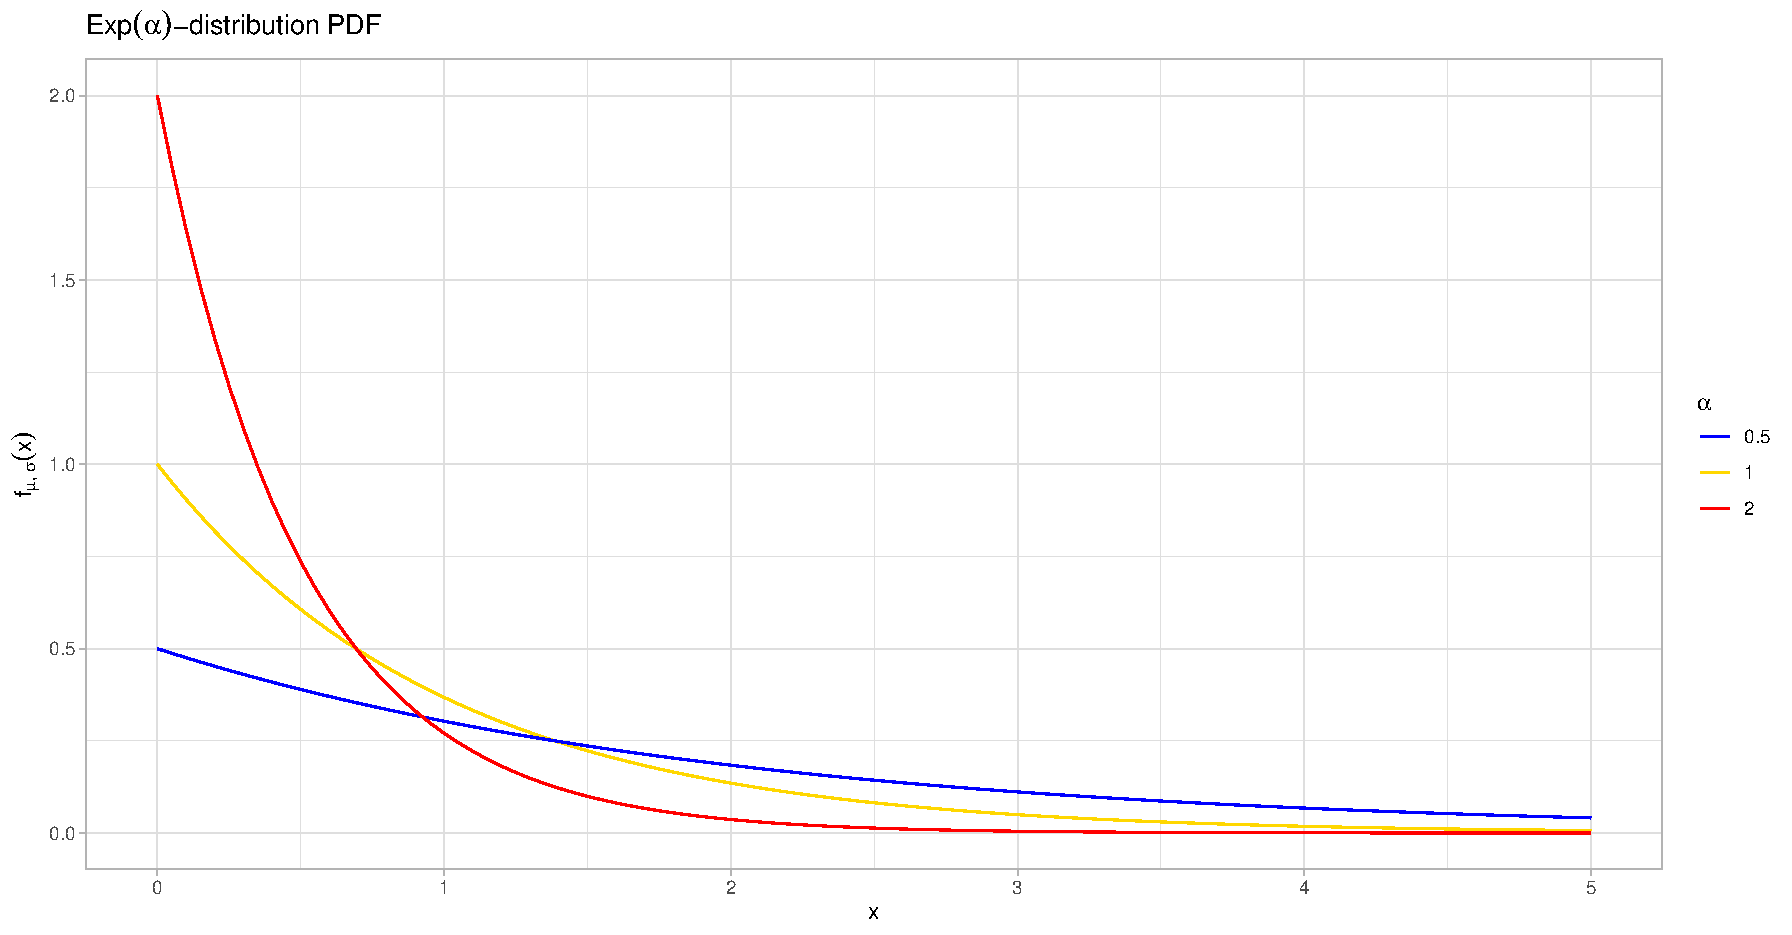
\includegraphics[width=1.0\linewidth]{material/exponential_PDF}
		\label{fig:exponential_PDF}
		&
		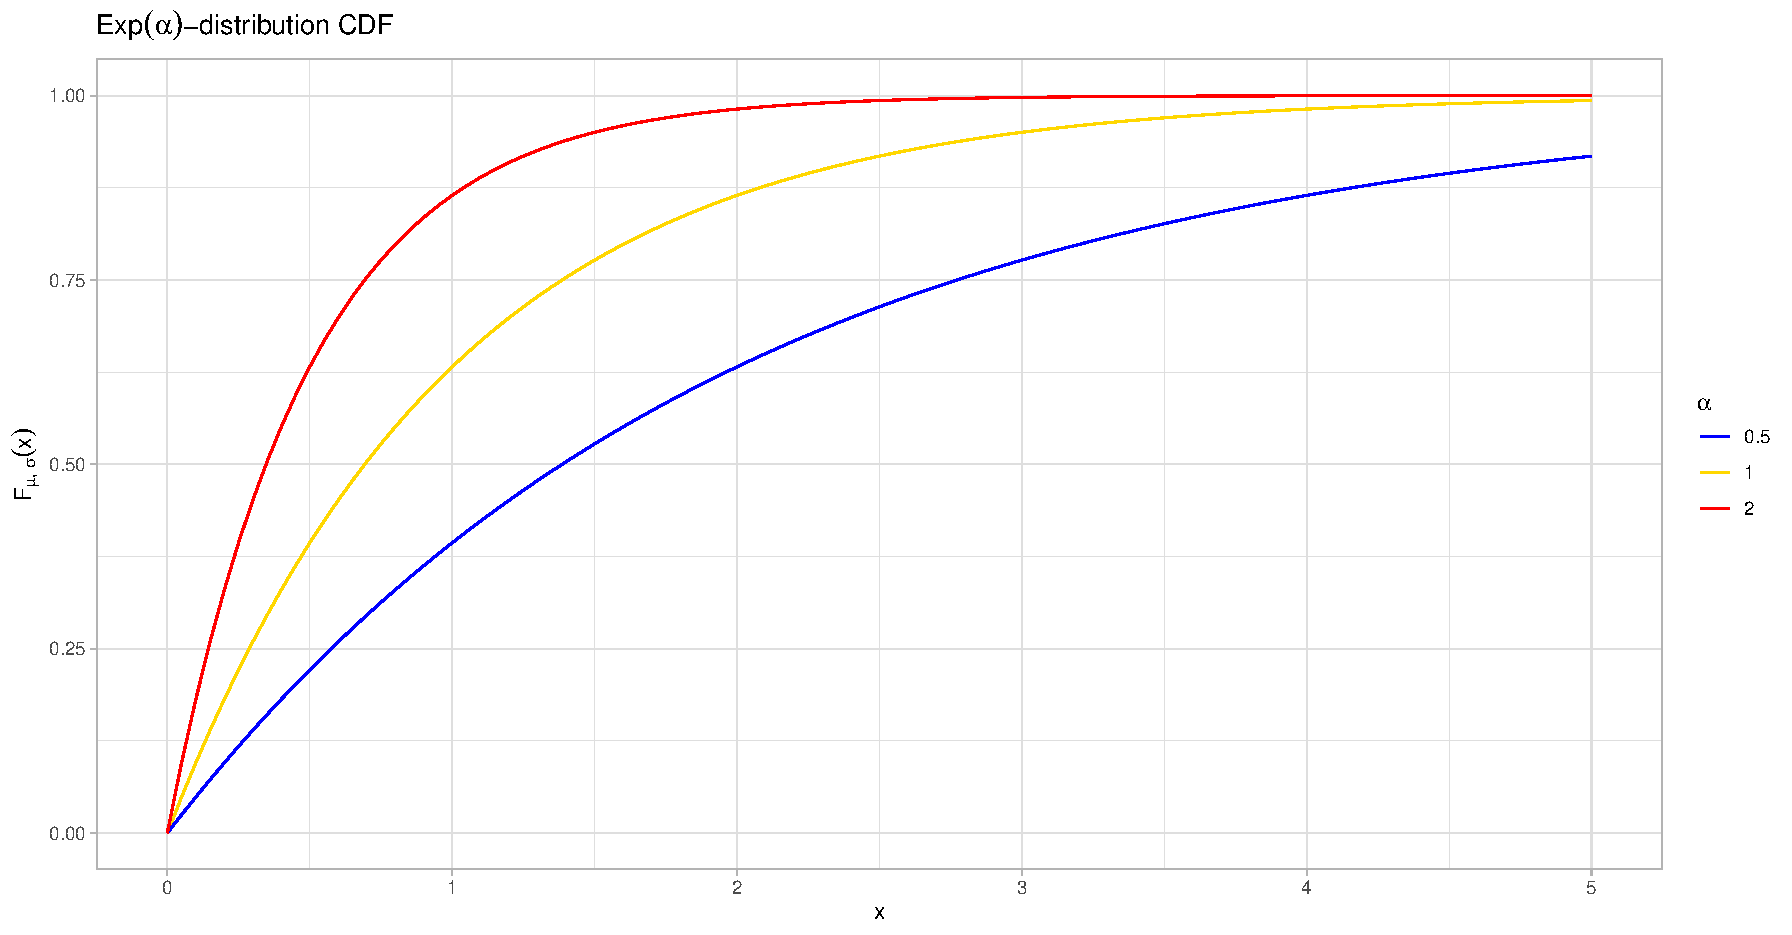
\includegraphics[width=1.0\linewidth]{material/exponential_CDF}
		\label{fig:exponential_CDF}
		\\
	\end{tabular} \\
	
	\vspace{-24pt}
	\begin{center}
		\begin{tabular}{|*3{>{\centering\arraybackslash}p{.3112\textwidth}|}}
			\hline
			Mean
			\[ E\left [ X \right ] = \frac{1}{\alpha} \]
			& Variance
			\[ \text{Var}\left( X\right) = \frac{1}{\alpha^{2}} \]
			& Fisher Information
			\[\mathcal{I} \left ( \theta \right ) = \frac{1}{\theta^{2}} \]
			\\
			\hline
		\end{tabular} \\
	\end{center}
	
	\vspace{-22.5pt}
	\begin{center}
		\begin{tabular}{|*2{>{\centering\arraybackslash}p{.48\textwidth}|}}
			\hline
			Moment-generating function
			\[ M_{X}\left( t\right) = \frac{\alpha}{\alpha -t} \]
			& Characteristic function
			\[ \varphi_{X}\left( t\right) = \frac{\alpha}{\alpha -it} \]
			\\
			\hline
		\end{tabular} \\
	\end{center}
	
	\vspace{-22.5pt}
	\begin{center}
		\begin{tabular}{|*1{>{\centering\arraybackslash}p{.9865\textwidth}|}}
			\hline
			Maximum Likelihood Estimator
			\[ \hat\alpha = \frac{n}{\sum_{i=1}^{n}x_{i}} \]
			\\
			\hline
		\end{tabular} \\
	\end{center}
	
	\begin{itemize}
		\item $P\left ( X\geq x+t \mid  X\geq x  \right ) = P\left ( X\geq t \right )$ (Memorylessness)
	\end{itemize}
	
	\newpage
		
	\subsection{Fisher($m$,$n$) distribution}
	\begin{tabular}{|*2{>{\centering\arraybackslash}p{.48\textwidth}|}}
		\hline
		Density
		\[ f \left ( x \right ) = \frac{\Gamma\left ( \frac{m+n}{2} \right ) \left ( \frac{m}{n} \right )^{\frac{m}{2}}}{\Gamma\left ( \frac{m}{2} \right ) \Gamma\left ( \frac{n}{2} \right )} x^{\left ( \frac{m}{2} - 1\right )} \left ( 1+\frac{m}{n} x \right )^{-\frac{m+n}{2}}
		\] 
		& Distribution function
		\[ - \]
		\\
		$\supp f\left( x\right) = \mathbb{R}^{+}_{0}$ &
		\\
		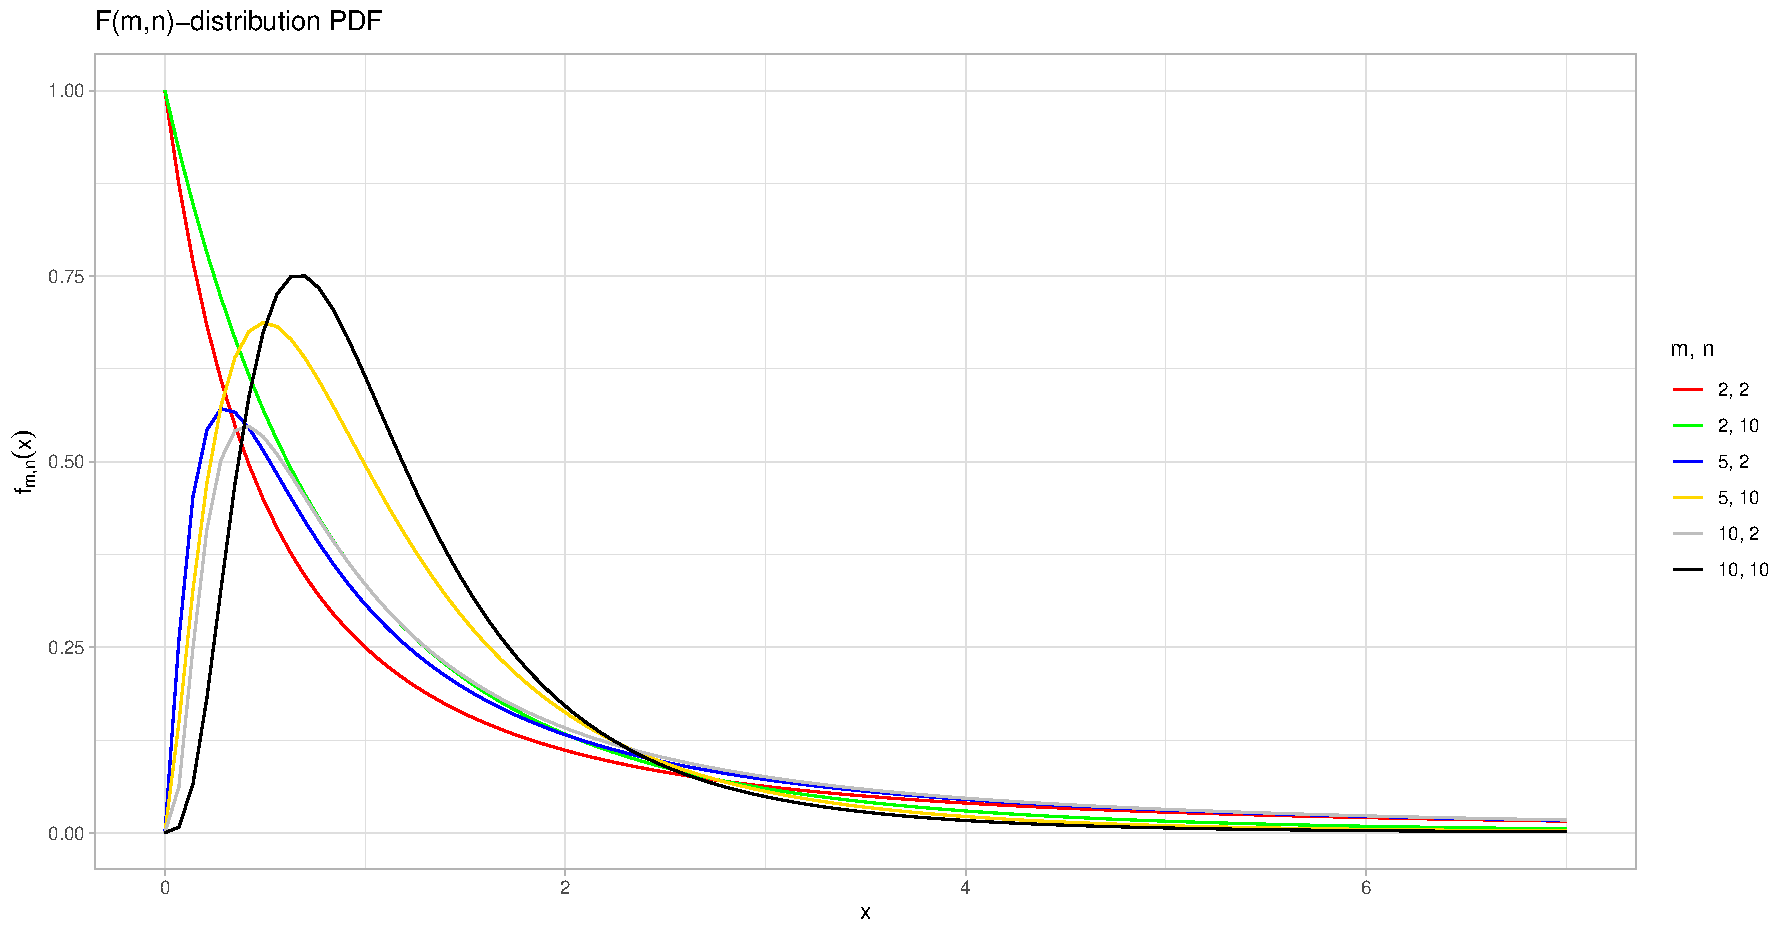
\includegraphics[width=1.0\linewidth]{material/fisher_PDF}
		\label{fig:fisher_PDF}
		&
		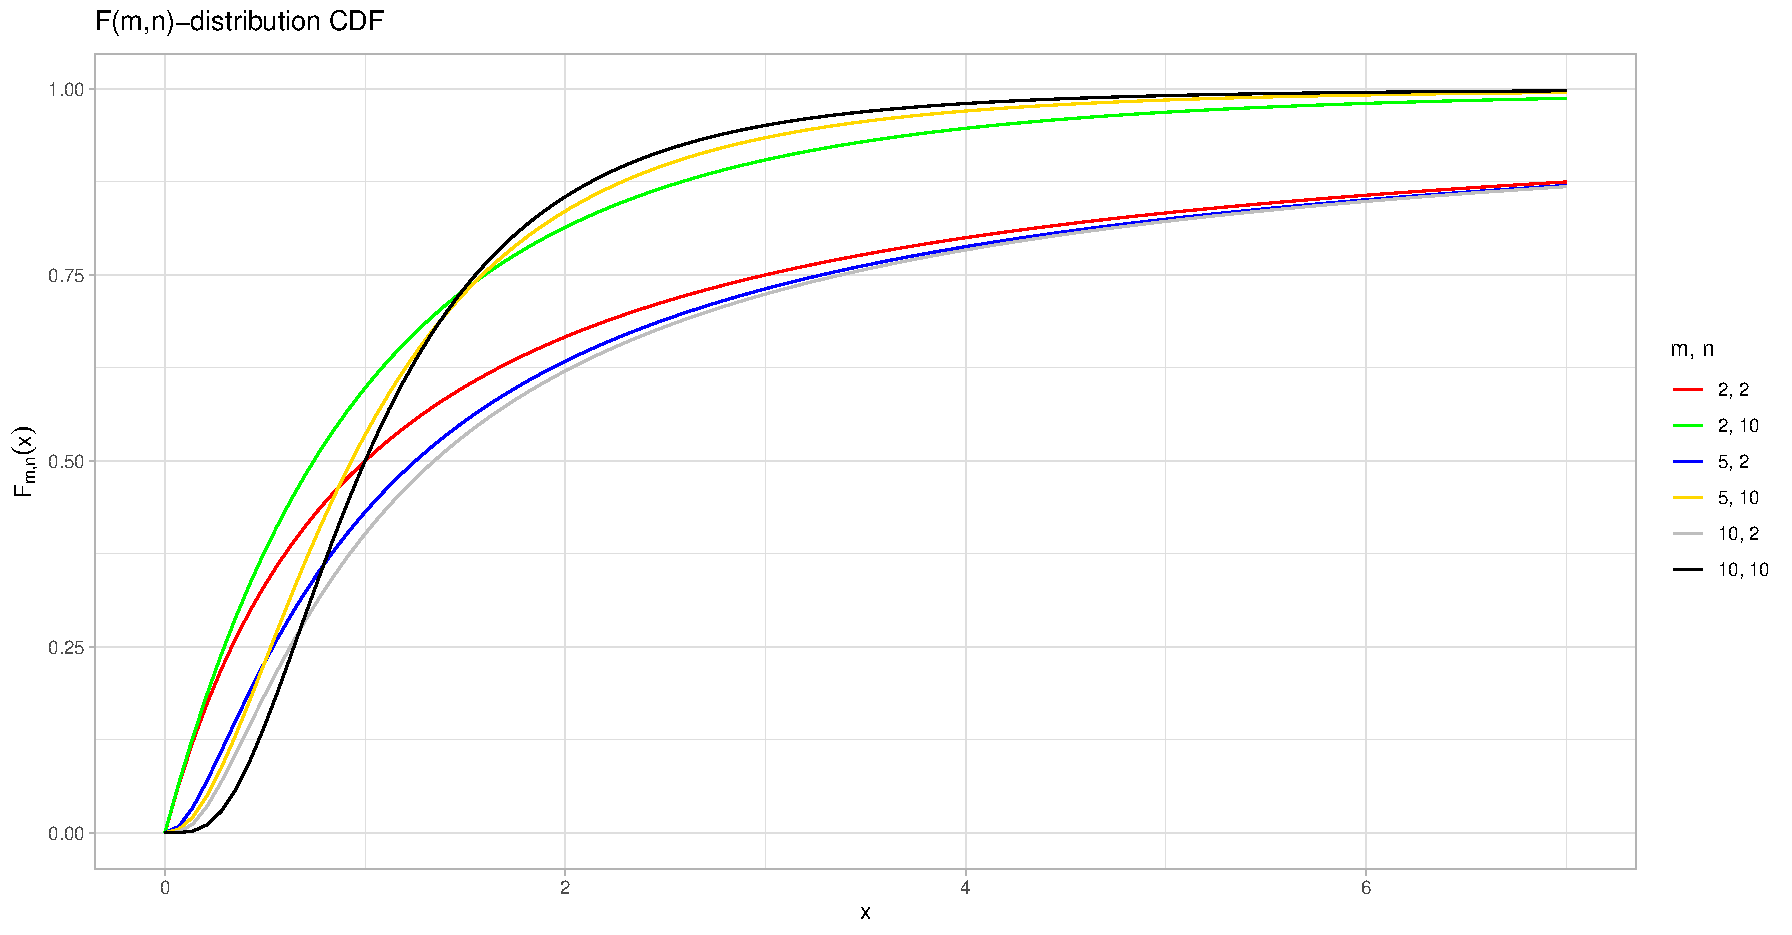
\includegraphics[width=1.0\linewidth]{material/fisher_CDF}
		\label{fig:fisher_CDF}
		\\
		\hline
		Mean
		\[ E\left [ X \right ] = \frac{n}{n-2} \]
		& Variance
		\[ \text{Var}\left( X\right) = \frac{2n^{2}\left( m+n-2\right) }{m\left( n-2\right) ^{2}\left( n-4\right) } \]
		\\
		\hline
	\end{tabular} \\
	
	\newpage
	
	\subsection{Student's($n$) distribution}
	\begin{tabular}{|*2{>{\centering\arraybackslash}p{.48\textwidth}|}}
		\hline
		Density
		\[ f \left ( x \right ) = \frac{\Gamma \left ( \frac{n+1}{2} \right )}{\Gamma\left ( \frac{n}{2} \right ) \sqrt{n \pi}} \left ( 1+\frac{x^{2}}{n} \right )^{-\frac{n+1}{2}}
		\] 
		& Distribution function
		\[ - \]
		\\
		$\supp f\left( x\right) = \mathbb{R}$ &
		\\
		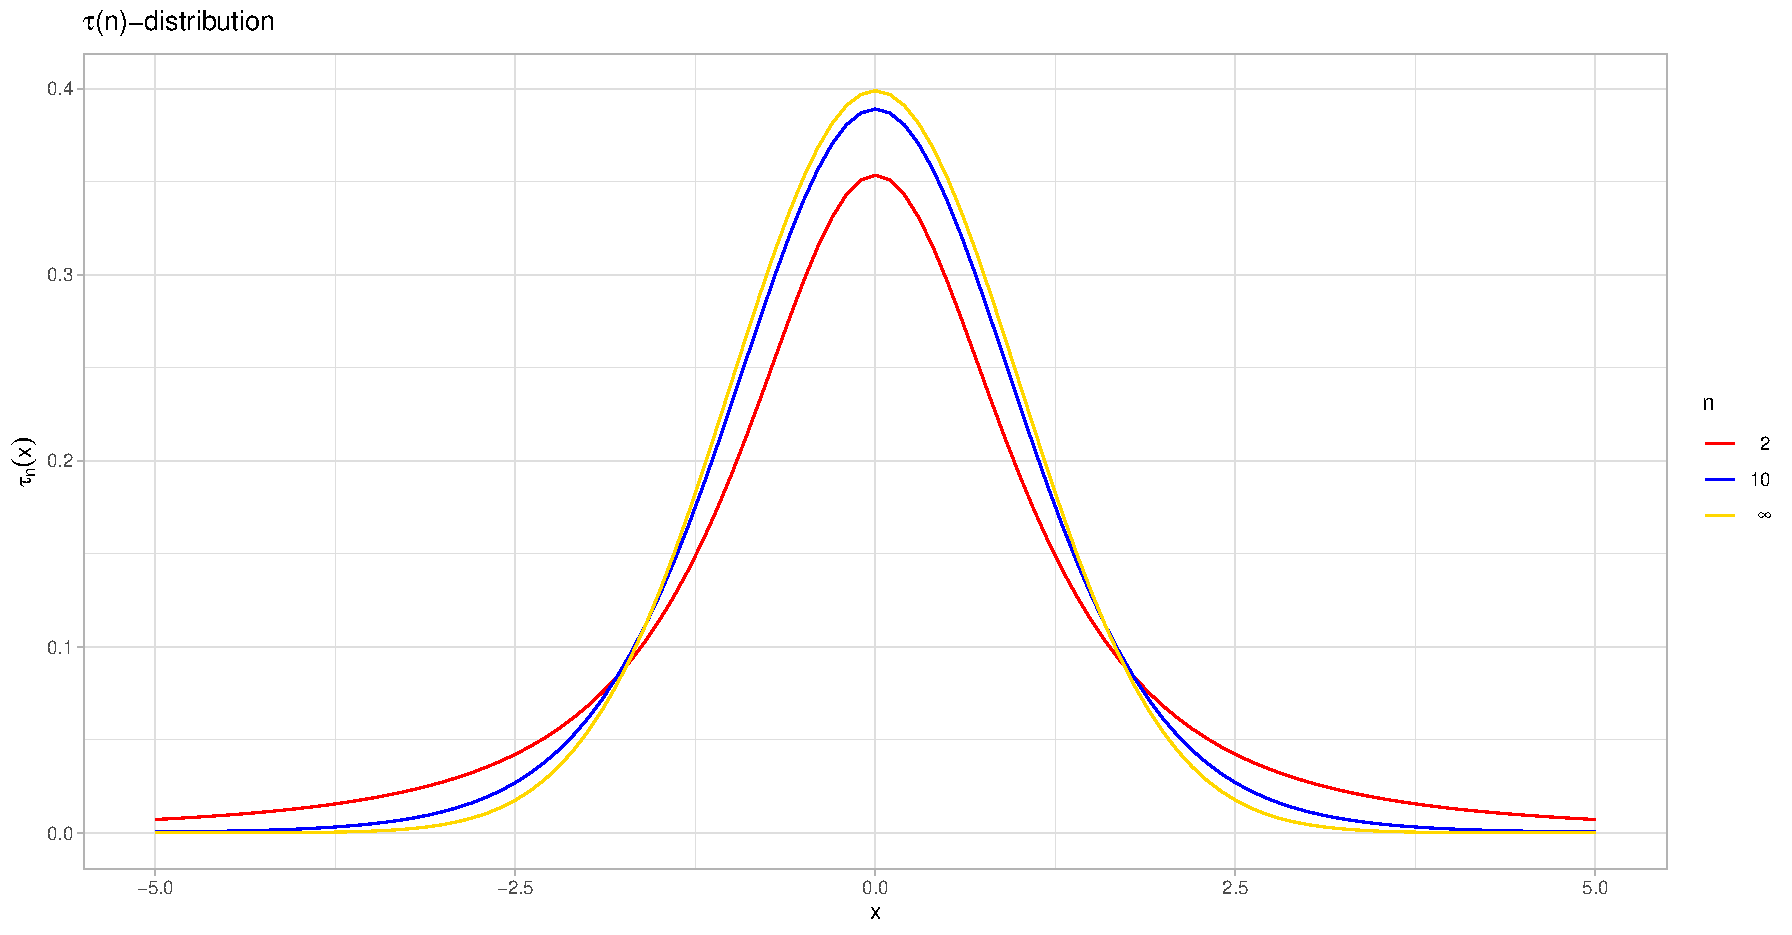
\includegraphics[width=1.0\linewidth]{material/student_PDF}
		\label{fig:student_PDF}
		&
		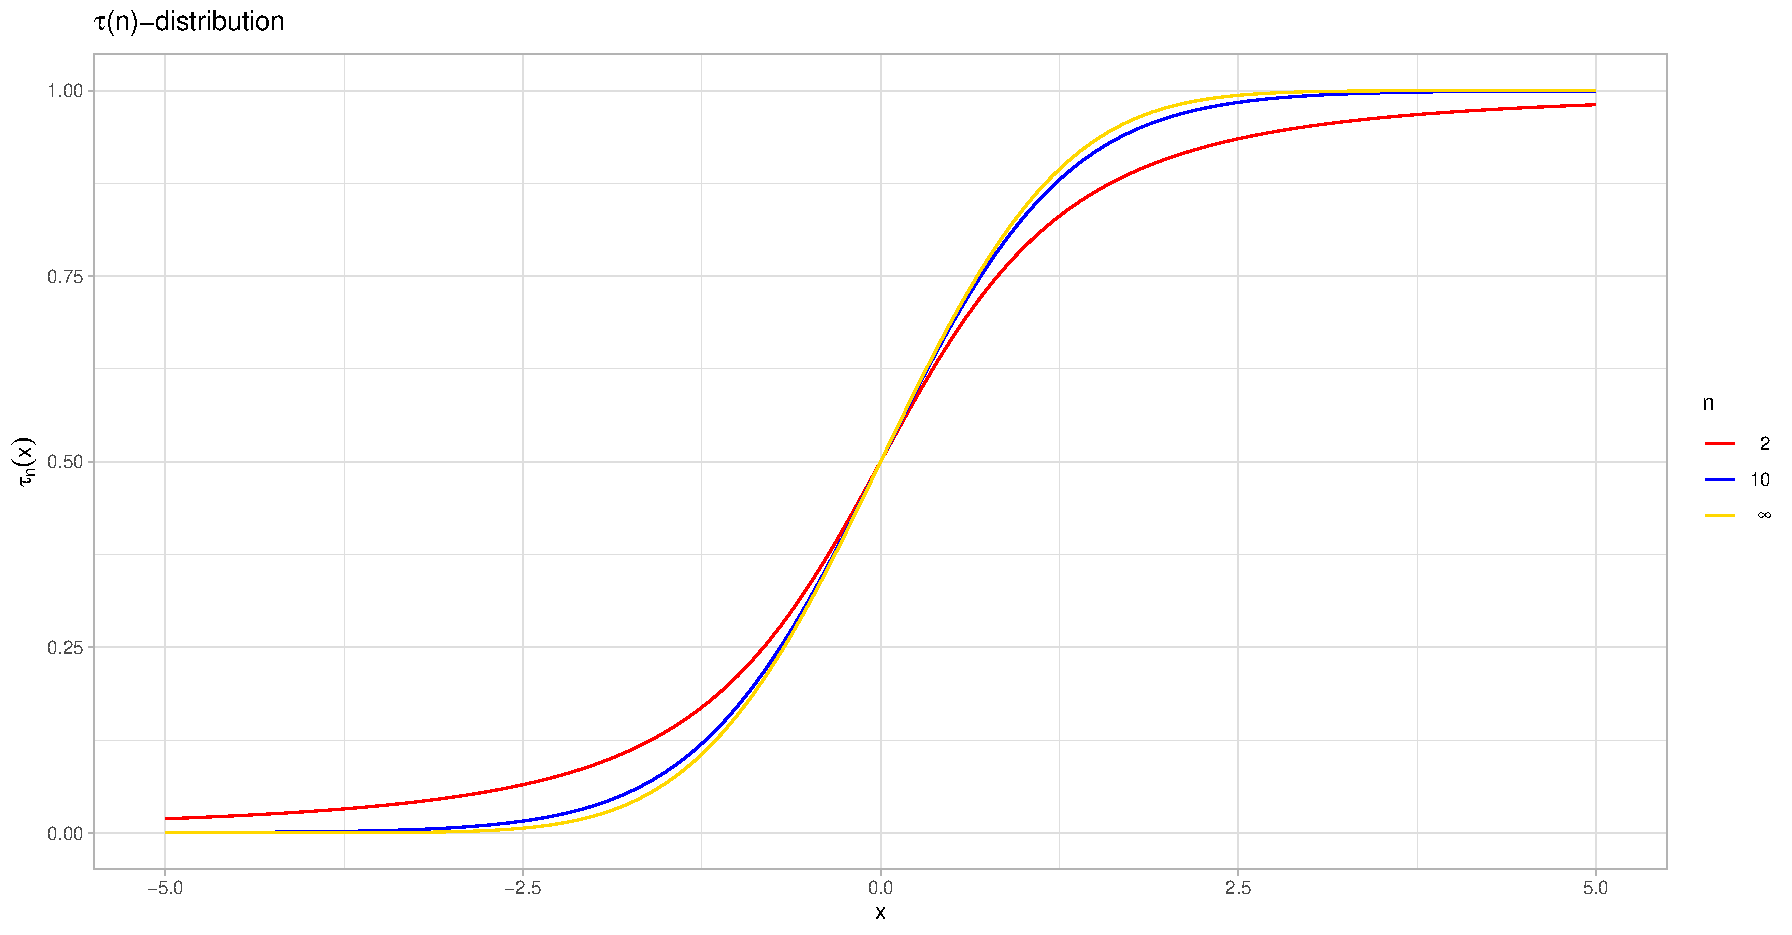
\includegraphics[width=1.0\linewidth]{material/student_CDF}
		\label{fig:student_CDF}
		\\
		\hline
		Mean
		\[ E\left [ X \right ] = 0 \]
		& Variance
		\[ \text{Var}\left( X\right) = \frac{n}{n-2} \]
		\\
		\hline
	\end{tabular}\\
	
	\begin{itemize}
		\item $\tau \left ( n \right ) = N\left ( 0,1 \right ) \text{ as } n \rightarrow \infty$
	\end{itemize}	
	
\end{document}